\chapter{Fundamentação Teórica}

\section{Linux Embarcado}

\subsection{\textit{Raspberry Pi 3 Model B+} - Versão Anatel}

O \textit{Raspberry Pi 3 Model B+} é um \textit{kit} de desenvolvimento que carrega como principal elemento o \textit{SOC} \textit{Broadcom BCM2837B0}.
O processador que esse \textit{SOC} carrega é um \textit{ARM Cortex-A53} com quatro núcleos \textit{64-bits} que rodam com um \textit{clock} de $1.4 GHz$ \cite{rasp3bplus2019}. 
Existe a versão do \textit{kit} de desenvolvimento homologada pela Anatel. A versão da placa homologada pela Anatel é azul como a Figura \ref{fig:rasp_anatel}. Essa versão homologada foi produto de uma parceria com a fundação do projeto Raspberry Pi com a revendedora de componentes eletrônicos catarinense Felipe Flop \cite{raspanatel2019}.

\begin{figure}[!htb]
    \centering
    \caption{\textit{Raspberry Pi 3 Model B+} - Versão Anatel.}
    \label{fig:rasp_anatel}
    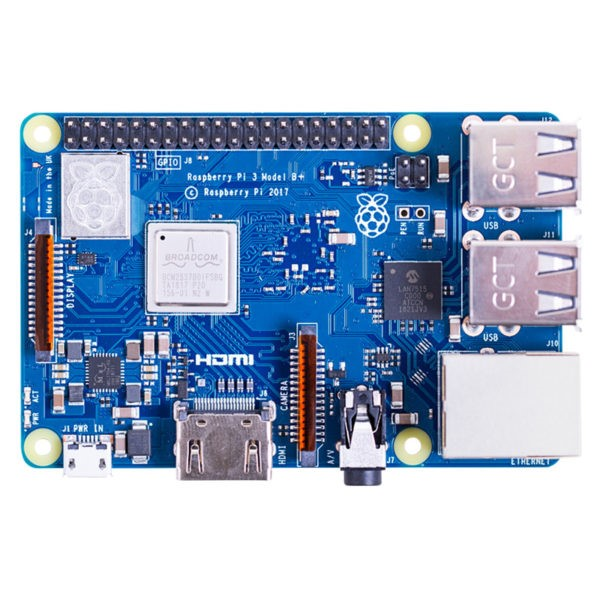
\includegraphics[width=0.6\textwidth]{./img/fundamentacao/rasp_anatel.jpg}
\end{figure}
Fonte: Filipe Flop

O \textit{SOC} \textit{Cypress CYW43455} é o componente encarregado pelo sistema de \textit{WIFI} e \textit{Bluetooth} 4.2. 
Esse componente fornece uma banda de $46.7Mb/s$ na transmissão de datos e $46.3Mb/s$ na recepção de dados com a frequência de portadora $2.4GHz$ e $102Mb/s$ transmissão e recepção de dados com frequência de portadora igual $5GHz$. 
O barramento do \textit{USB} 2.0 e a rede \textit{10/100 Ethernet} é responsabilidade do componente \textit{LAN7515} da \textit{Microchip}. As velocidades levantadas pelo fabricante do \textit{Raspberry Pi} para esse barramento de $315Mb/s$  com frequência de portadora igual $5GHz$ \cite{rasp3bplus2019}.
 
 \pagebreak
 
\subsection{Ubuntu Mate 18.04 e Raspberry Pi}
O \textit{Ubuntu MATE 18.04 (Bionic Beaver) Beta 1}, avaliado para \textit{Raspberry Pi Model B 2}, \textit{3} and \textit{3+}, é disponibilizado na forma já compilada para as arquiteturas \textit{armhf (ARMv7 32-bit)} e \textit{arm64 (ARMv8 64-bit)}.
Esse sistema provê, além dos \textit{drivers} para \textit{Ethernet}, \textit{WIFI} e \textit{Bluetooth}, acesso ao \textit{GPIO} via \textit{GPIO Zero}, \textit{pigpio} e \textit{WiringPi} \cite{wimpress2019}.   

\subsection{\textit{ROS Melodic Morenia} e \textit{Ubuntu Mate 18.04}}

O \textit{ROS Melodic Morenia} é direcionado principalmente para a versão \textit{Ubuntu 18.04 (Bionic)}, embora outros sistemas \textit{Linux} e \textit{Mac OS X}, \textit{Android} e \textit{Windows} sejam suportados em vários graus \cite{rosmelodic2019}.
Logo o \textit{Ubuntu Mate 18.04} se mostra uma boa alternativa para o uso do sistema \textit{ROS} junto ao\textit{raspberry Pi 3 Model B+}.

\subsection{Configuração do modo \textit{Access Point}} - \textit{Netplan}
O \textit{Netplan} é o \textit{software} nativo do \textit{Ubuntu Mate 18.04}.
Com um arquivo de configuração de extensão \textit{.yaml}, por meio desse \textit{software}, é possível configurar o  

\subsection{\textit{Python} Embarcado}

\subsection{\textit{OpenSSH-server}}

\pagebreak

\section{\textit{OpenCV}}
A biblioteca de \textit{software} \textit{OpenCV} (\textit{Open Source Vision Library}) é uma biblioteca de código aberto desenvolvida pela comunidade afim de otimizar o processo de produção de \textit{softwares} de processamento de imagem. Essa biblioteca conta com mais de 2500 algorítimos otimizados de visão computacional e \textit{machine learning}.
Essa biblioteca é amplamente utilizada em empresas como \textit{Google}, \textit{Yahoo}, \textit{Microsoft}, \textit{Intel}, \textit{IBM}, \textit{Sony}, \textit{Honda}, \textit{Toyota} \cite{aboutopencv2019}. Sendo um produto de licença do tipo \textit{BSD-licensed} é uma alternativa para desenvolvimento de produtos comerciais \cite{opensource2019}.
    
Essa biblioteca é escrita nativamente em \textit{C++}, porém fornece interfaces para as linguagens de programação \textit{C++}, \textit{Python}, \textit{Java} e \textit{Matlab} e da suporte para os sistemas operacionais \textit{Windows}, \textit{Linux}, \textit{Mac OS} e \textit{Android}.  

\subsection{Compilação do \textit{OpenCV}}

\begin{itemize}
    \item \textbf{Ferramentas para compilação:} \textit{build-essential}, \textit{cmake}, \textit{unzip} e \textit{pkg-config}.
    \item \textbf{Bibliotecas de vídeo e imagem:} \textit{libjpeg-dev}, \textit{libpng-dev}, \textit{libtiff-dev}, \textit{libavcodec-dev}, \textit{libavformat-dev},  \textit{libswscale-dev}, \textit{libv4l-dev}, \textit{libxvidcore-dev} e \textit{libx264-dev}.
    \item \textbf{GUI-\textit{Backend}:} \textit{libgtk-3-dev} e \textit{libcanberra-gtk*}.
    \item \textbf{Otimização Numérica:} \textit{libatlas-base-dev} e \textit{gfortran}.
    \item \textbf{Arquivos de cabeçalho para criação de pacotes python:} \textit{python3-dev}.
\end{itemize}

\cite{rosebrock2018}

% Ferramentas para compilação:\
% $$ \$ sudo apt-get install build-essential cmake unzip pkg-config $$
% Next, let’s install a selection of image and video libraries — these are critical to being able to work with image and video files:
% $$ \$ sudo apt-get install libjpeg-dev libpng-dev libtiff-dev $$
% $$ \$ sudo apt-get install libavcodec-dev libavformat-dev libswscale-dev libv4l-dev $$
% $$ \$ sudo apt-get install libxvidcore-dev libx264-dev $$
% From there, let’s install GTK, our GUI backend:
% $$ \$ sudo apt-get install libgtk-3-dev $$

\pagebreak

\subsection{\textit{OpenCV} - \textit{Python}}
Todos os algorítimos da biblioteca \textit{OpenCV} são implementados com a linguagem de programação \textit{C++}. 
Porém a programação dessa biblioteca com o uso de outras linguagens de programação se faz possível por meio de um mecanismo que a documentação do \textit{OpenCV} intitula como \textit{bindings generator}. 
Esse gerador é responsável por gerar um mecanismo que possibilita ao interpretador \textit{Python} fazer chamadas de funções já compiladas que foram escritas com a linguagem \textit{C++}.
Essas pontes (\textit{bindings}) poderiam ser programadas manualmente, uma a uma, por um programador. 
Porém pelo fato da biblioteca conter mais de 2500 funções \cite{aboutopencv2019}, a programação manual dessas pontes se torna uma tarefa demasiadamente exaustiva.
A forma que os desenvolvedores do \textit{OpenCV} adotaram para viabilizar a criação de todas as pontes, uma para cada função da biblioteca, foi a automatização do processo. 
Um \textit{script} escrito com a linguagem de programação \textit{python} faz a leitura de todos os arquivos de cabeçalhos (\textit{headers}) da biblioteca \textit{OpenCV} escrita em \textit{C++} e gera uma ponte (\textit{binding}) para cada função da biblioteca\cite{opencvpython2019}.
Dessa forma é possível utilizar da eficiência de uma função já compilada junto a praticidade de uma linguagem interpretada.
  
\pagebreak

\section{\textit{ROS}}

O sistema \textit{ROS}, \textit{Robot Operating System} é um  \textit{frameworks} para desenvolvimento de robôs. O \textit{ROS} fornece a funcionalidade de um sistema operacional que é capaz de operar múltiplos computadores heterogêneo \cite{aboutros2019}. Isso é pertinente para atender os objetivos específicos desse trabalho referentes a comunicação \textit{TCP/IP}.
O sistema \textit{ROS} é inicialmente composto por um nó central acionado pelo comando \textit{roscore}.
Após a inicialização desse nó central, mais nós podem ser iniciados formando uma rede com protocolo \textit{TCP/IP}.
Esses nós podem rodar dentro de um mesmo computador ou em diferentes computadores.
O nó central, iniciado pelo comando \textit{roscore}, é responsável por gerir a rede, e quando ele é desativado, todos os nós são desativados. 

A Figura \ref{fig:roscore} mostra a saída do programa \textit{roscore}. Ou seja, a mensagem que o programa escreve após sua execução. 
No caso do sistema utilizado nesse trabalho, a sua distribuição é chamada de \textit{Melodic Morenia 1.14.3}. 
Essa é a décima segunda versão. 
Sua data de lançamento foi 23 de maio de 2018 \cite{rosmelodic2019}.
De ano em ano uma distribuição é lançada e essa recebe suporte técnico de 5 anos \cite{rosdist2019}.
Na Figura \ref{fig:roscore} também é possível ver também o endereço do nó principal: \textbf{ROS\_MASTER\_URI=http://lucas-K46CA:11311/} e o \textit{pid} do processo.

\begin{figure}[!htb]
    \centering
    \caption{Comando \textit{roscore} - Inicialização do nó principal da rede ROS.}
    \label{fig:roscore}
    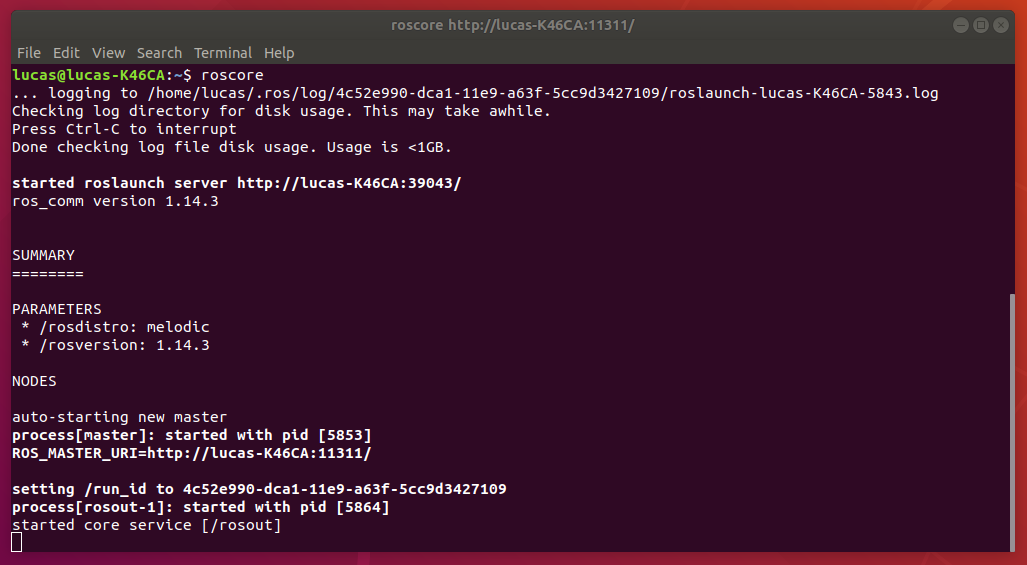
\includegraphics[width=\textwidth]{./img/fundamentacao/roscore.png}
\end{figure}
Fonte: Autor

\pagebreak

Sendo a ideia do \textit{ROS} a operação de vários nós em uma rede operando com protocolo \textit{TCP/IP}, cada nó acaba recebendo uma identificação. 
Considerando uma exemplificação adaptada de \citeonline{fernandes2019}, onde uma rede com três nós está operando, o comando \textit{rosnode list} tem como saída a listagem do nome dos três nós em operação. 
A Figura \ref{fig:rosnode_list} mostra saída do comando \textit{rosnode list}. 
A listagem dos três nós, sendo o nó com nome \textbf{\textit{/talker}} programado para enviar mensagens, o nó com nome \textbf{\textit{/listener}} programado para escutar mensagens e o nó com nome \textbf{\textit{/rosout}} é o \textit{console log reporting}. 
Esse é responsável por publicar e receber mensagem do sistema. 
O nó \textbf{\textit{/rosout}} sempre é iniciado com o comando \textit{roscore}.

\begin{figure}[!htb]
  \centering
  \caption{Comando \textit{rosnode list} - lista os nós ativos.}
  \label{fig:rosnode_list}
  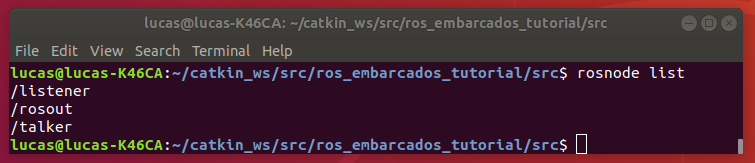
\includegraphics[width=0.9\textwidth]{./img/fundamentacao/rosnode_list.png}
\end{figure}

Fonte: Autor

Os nós podem interagir entre si por meio de mensagens escritas em tópicos (\textit{topics}) ou por meio de \textit{services} que alguns nós venham a fornecer.
Os tópicos são uma abstração de locais na rede onde é possível publicar ou ler mensagens. 
A Figura \ref{fig:rostopic_list} mostra como a execução do comando \textit{rostopic list} mostra todos os tópicos ativos. 
No caso, o nó \textit{/talker} é programado para escrever no tópico \textit{/chatter} enquanto o nó \textit{listener} é programado para ler o tópico \textit{/chatter}. 
Dessa forma o nó \textit{/talker} pode enviar mensagens de maneira assíncrona para o nó \textit{/listener}.

\begin{figure}[!htb]
  \centering
  \caption{Comando \textit{rostopic list} - lista os tópicos ativos.}
  \label{fig:rostopic_list}
  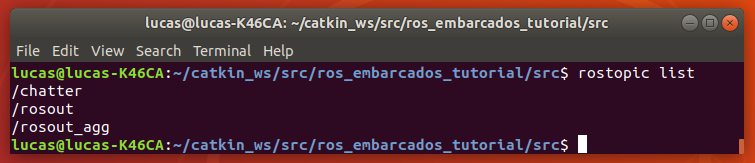
\includegraphics[width=0.9\textwidth]{./img/fundamentacao/rostopic_list.png}
\end{figure}

Fonte: Autor

Por meio da abstração dos tópicos é possível definir a rota das mensagens pela rede. Vale ressaltar que um tópico é uma abstração. 
As mensagens não são enviadas a um tópico com endereço específico na rede. 
As mensagens são enviadas diretamente de um nó a outro. 
Os tópicos servem para facilitar a descrição do fluxo de dados da rede.

\pagebreak

O comando \textbf{\textit{rosnode info /roscore}}, como indicado na Figura \ref{fig:rosnode_info_rosout}, tem como saída informações pertinentes sobre cada nó, no caso o nó \textit{/roscore}.
Em \textit{Publications} é indicado em quais tópicos esse nó escreve mensagens e em \textit{Subscriptions} é indicado em quais tópicos esse nó lê mensagens.
Dessa forma é possível ver que o nó \textit{/rosout} está inscrito no tópico \textit{/rosout} (que possui o mesmo nome) e publica mensagens no tópico \textit{/rosout\_agg}.
Também é possível visualizar o tipo da mensagem que o tópico utiliza pois esse é tipado (o dado possui formato específico).
No caso do tópico \textit{/rosout}, esse opera com mensagens do tipo \textit{rosgraph\_msgs/Log}.

Como mencionado anteriormente, além da escrita em tópicos, uma outra forma dos nós interagirem é por meio dos \textit{services}. 
A Figura \ref{fig:rosnode_info_rosout} mostra os \textit{services} disponíveis pelo nó \textit{/rosout}. 
O \textit{get\_logger} e \textit{set\_logger\_level} são \textit{services} pertencentes ao nó \textit{/rosout} que podem ser acionados a qualquer momento.
Esses dois \textit{services} em específico são utilizados para depuração.

\begin{figure}[!htb]
  \centering
  \caption{Comando \textit{rosnode info /rosout} - Informações sobre o nó \textit{/rosout}.}
  \label{fig:rosnode_info_rosout}
  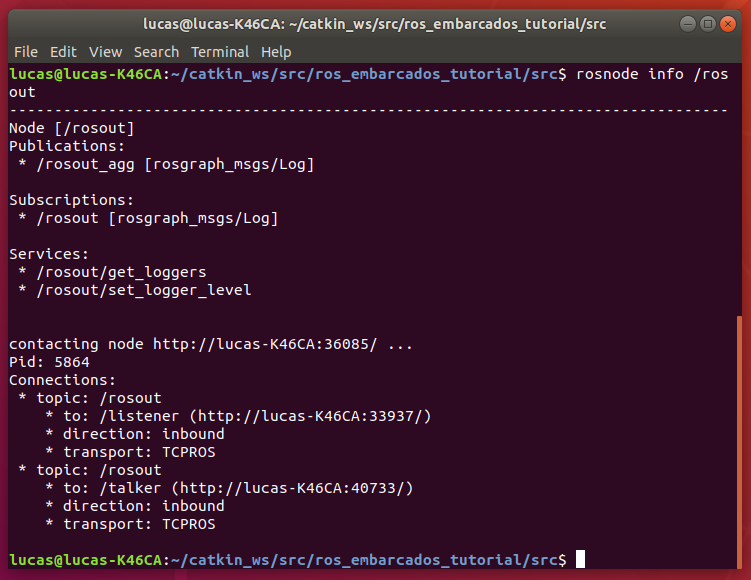
\includegraphics[width=0.9\textwidth]{./img/fundamentacao/rosnode_info_rosout.png}
\end{figure}
Fonte: Autor


Também é disposta todas as conexões que esse nó estabelece, na parte indicada com a palavra \textit{Connections} na Figura \ref{fig:rosnode_info_rosout}. 
É possível ver que o nó central se conecta tanto com o nó \textit{/listener} quanto com o nó \textit{/talker}, pelo tópico \textit{/rosout}. 
Também é indicado a direção da mensagem (\textit{inbound} significa que o nó recebe a mensagem) e o protocolo de transporte da mensagem, que no caso é uma variação do TCP/IP, o TCPROS.

\pagebreak

O comando \textbf{\textit{rosnode info /talker}} por sua vez mostra as informações do nó \textit{/talker}.
Na Figura \ref{fig:rosnode_info_talker} é possível verificar que esse nó escreve nos tópicos \textit{/chatter} e \textit{/rosout}. 
Diferente do nó \textit{/rosout} que lê as mensagens do tópico \textit{/rosout}, o nó \textit{/talker} escreve mensagens no tópico.
Logo o campo \textit{direction} está indicando \textit{outbound}, diferente do caso do nó \textit{/rosout}, Figura \ref{fig:rosnode_info_rosout}, que estava indicando \textit{inbound}.
A Figura \ref{fig:talker_rosnode_info_connect} mostra o grafo montado com as informações apresentadas na Figura \ref{fig:rosnode_info_talker}.

\begin{figure}[!htb]
  \centering
  \caption{Comando \textit{rosnode info /talker} - Informações sobre o nó \textit{/talker}.}
  \label{fig:rosnode_info_talker}
  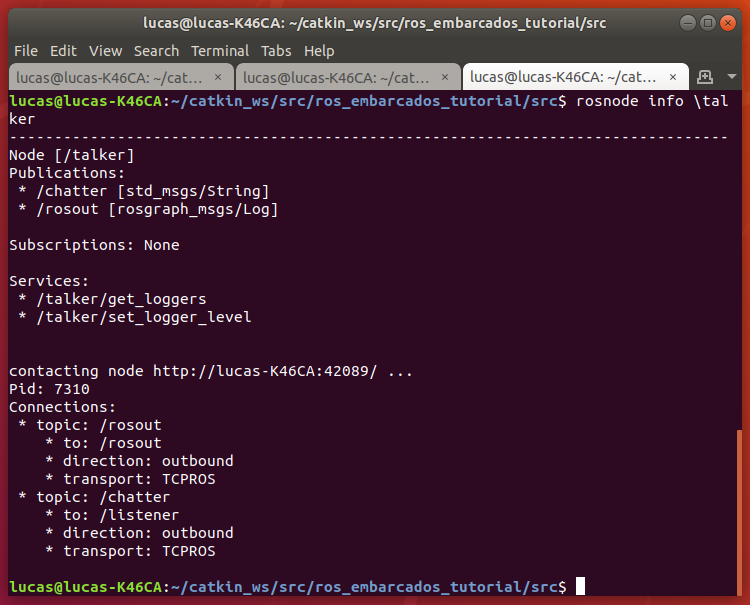
\includegraphics[width=0.8\textwidth]{./img/fundamentacao/rosnode_info_talker.png}
\end{figure}
Fonte: Autor

\begin{figure}[!htb]
  \centering
  \caption{Conexões do nó \textit{/talker}.}
  \label{fig:talker_rosnode_info_connect}
  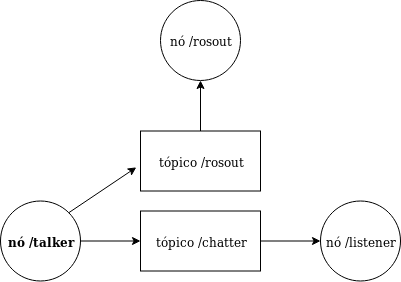
\includegraphics[width=0.50\textwidth]{./img/fundamentacao/talker_rosnode_info_connect.png}
\end{figure}
Fonte: Autor

\pagebreak

Com o comando \textbf{\textit{rosnode info /listener}} é possível extrair as mesmas informações apresentadas na Figura \ref{fig:rosnode_info_talker}, só que agora referentes ao nó \textit{/listener}. 
Dessa vez o campo \textit{direction} do tópico \textit{/chatter} está indicando \textit{inbound}. Isso significa que, diferente do nó \textit{/talker}, o nó \textit{/listener} lê mensagens do tópico \textit{/chatter}.

\begin{figure}[!htb]
  \centering
  \caption{Comando \textit{rosnode info /listener} - Informações sobre o nó \textit{/listener}.}
  \label{fig:rosnode_info_listener}
  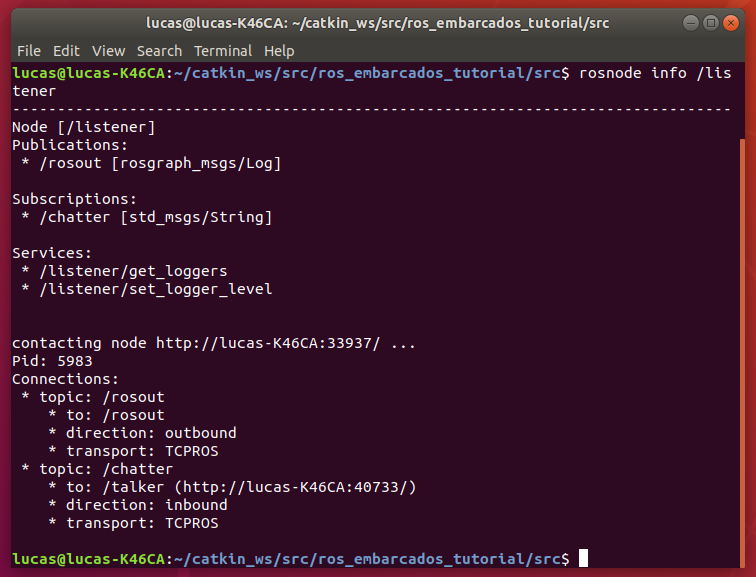
\includegraphics[width=0.8\textwidth]{./img/fundamentacao/rosnode_info_listener.png}
\end{figure}
Fonte: Autor

Com as informações apresentadas na Figura \ref{fig:rosnode_info_rosout}, Figura \ref{fig:rosnode_info_talker} e Figura \ref{fig:rosnode_info_listener} é possível montar o grafo completo da rede (Figura \ref{fig:rosnet_listener_talker}).
Dessa forma resumidamente é demostrada de forma básica, por meio da exemplificação anterior, a lógica de funcionamento do ROS.

\begin{figure}[!htb]
  \centering
  \caption{Rede Completa.}
  \label{fig:rosnet_listener_talker}
  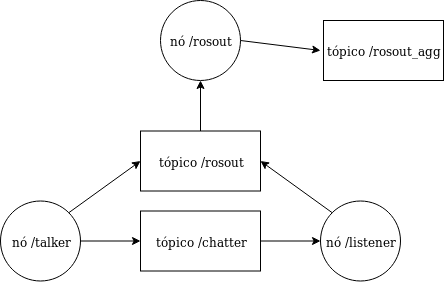
\includegraphics[width=0.50\textwidth]{./img/fundamentacao/rosnet_listener_talker.png}
\end{figure}
Fonte: Autor

\pagebreak

\subsection{ROS - TCP/IP - TCPROS}

A camada de transporte é chamada de TCPROS.
Nessa camada é utilizado o protocolo TCP/IP para transporte de mensagens via \textit{socket} \cite{tcpros2019}.
O ROS atualmente suporta protocolos do tipo TCP-IP e UDP-IP para estabelecer a comunicação entre nós \cite{rostopic2019}. 
E as mensagens são roteadas até o destino correto pelas informações contidas no \textit{TCPROS Header Field}.

\subsection{ROS - ROSSERIAL}

O pacote ROSSERIAL possibilita o uso de protocolo serial entre nós de uma rede ROS.
Esse pacote cria uma ponte entre o protocolo TCPROS(TCP/IP) e o protocolo serial. 
Dessa forma é possível trocar mensagens por meio de \textit{sockets} de rede \cite{fernandes_rosserial2019}. 
Atualmente o pacote ROSSERIAL fornece os seguintes suportes\cite{rosserial2019}:
\begin{itemize}
    \item \textbf{rosserial\_arduino} - suporte para plataforma Arduino.
    \item \textbf{rosserial\_embeddedlinux} - suporte para sistemas com Linux Embarcado (ex: Roteadores).
    \item \textbf{rosserial\_windows} - suporte para aplicações \textit{Windows}.
    \item \textbf{rosserial\_mbed} - suporte para plataforma \textit{Mbed}.
    \item \textbf{rosserial\_tivac} - suporte para a plataforma \textit{TI's Launchpad}.
    \item \textbf{rosserial\_vex\_v5} - suporte para o módulo \textit{VEX V5 Robot Brain}.
    \item \textbf{rosserial\_vex\_cortex} - suporte para o módulo \textit{VEX Cortex}.
    \item \textbf{rosserial\_stm32} - suporte para microcontroladores da linha \textit{STM32}.
    \item \textbf{ros-teensy} - suporte para a plataforma \textit{Teensy}.
\end{itemize}

Para o caso do uso da plataforma Arduino, que fonece suporte para o microcontrolador \textit{ATMEGA328P}, é compilada uma biblioteca que pode ser utilizada \cite{fernandes_rosserial2019}. 
Com um nó operando em um \textit{ATMEGA328P} é possível publicar em 25 tópicos diferentes e monitorar outros 25 tópicos. 
Dessa forma consumindo 560 bytes de memória (considerando os 50 tópicos - 25 para publicação e 25 para receber mensagens) \cite{arduinoros2019}. 

\pagebreak

\subsection{ROS e OpenCV}



\pagebreak
% \subsection{ROS - Python}

% \pagebreak

% \section{ROS e OpenCV}

% \pagebreak

% \pagebreak

% \section{HOG}

\section{Visão Estéreo}

Quando duas câmeras alinhadas capturam a imagem de um mesmo objeto, a disparidade da posição ocupada pelo objeto em cada sensor está relacionada com a profundidade do mesmo.
A Figura \ref{fig:stereo_vision_main_example} ilustra geometricamente como a disparidade das posições ocupadas nos sensores por um mesmo ponto pertencente ao seguimento $Z_d$ revela a profundidade do mesmo \cite{Kyto2011}.
Logo existe uma relação derivada do alinhamento entre todos os pontos da profundidade $Z_d$ com ponto de foco $f_L$ e todos os pontos do seguimento $Z_L$ no sensor ótico.

\begin{itemize}
    \item \textbf{$Z_d$}: Profundidade a ser medida.
    \item \textbf{$Z_R$}: Projeção de $Z_{d}$ no sensor ótico \textbf{direito} - \textit{Right}.
    \item \textbf{$Z_L$}: Projeção de $Z_{d}$ no sensor ótico \textbf{esquerdo} - \textit{Left}.
    \item \textbf{$f_R$}: Ponto focal da câmera \textbf{direita} - \textit{Right}.
    \item \textbf{$f_L$}: Ponto focal da câmera \textbf{esquerda} - \textit{Left}.
    \item \textbf{$b$}: Distância entre os pontos focais - \textit{baseline}.
\end{itemize}

\begin{figure}[!htb]
  \centering
  \caption{Sistema Estereoscópico.}
  \label{fig:stereo_vision_main_example}
  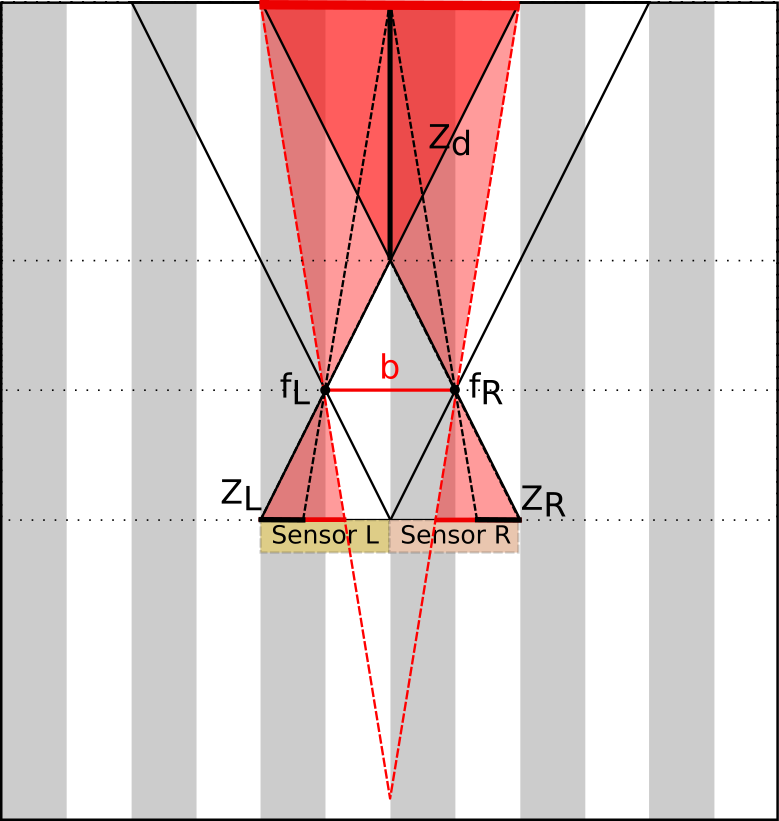
\includegraphics[width=0.65\textwidth]{./img/fundamentacao/stereo_vision_main_example.png}
\end{figure}
Fonte: Autor

\pagebreak

\subsection{Oclusão no contexto da visão estéreo.}

\ref{fig:stereo_vision_occlusion}
\begin{figure}[!htb]
  \centering
  \caption{Zona de oclusão.}
  \label{fig:stereo_vision_occlusion}
  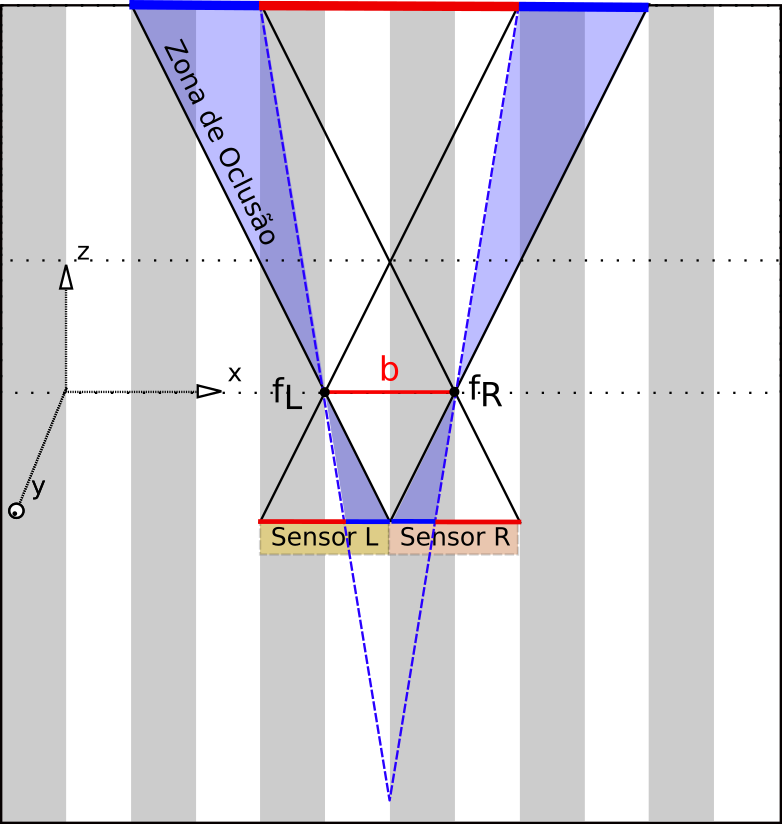
\includegraphics[width=0.7\textwidth]{./img/fundamentacao/stereo_vision_occlusion.png}
\end{figure}
Fonte: Autor

\pagebreak

\subsection{Resolução de profundidade em função da distância focal.}

\ref{fig:stereo_vision_focal_variation}

$$dZ_d = \frac{Z^2}{f_{L, R}b}dp_x$$
$$dp_x = \frac{1}{2 tan(FOV)} S_w \Delta T$$

\begin{figure}[!htb]
  \centering
  \caption{Variação da distância focal.}
  \label{fig:stereo_vision_focal_variation}
  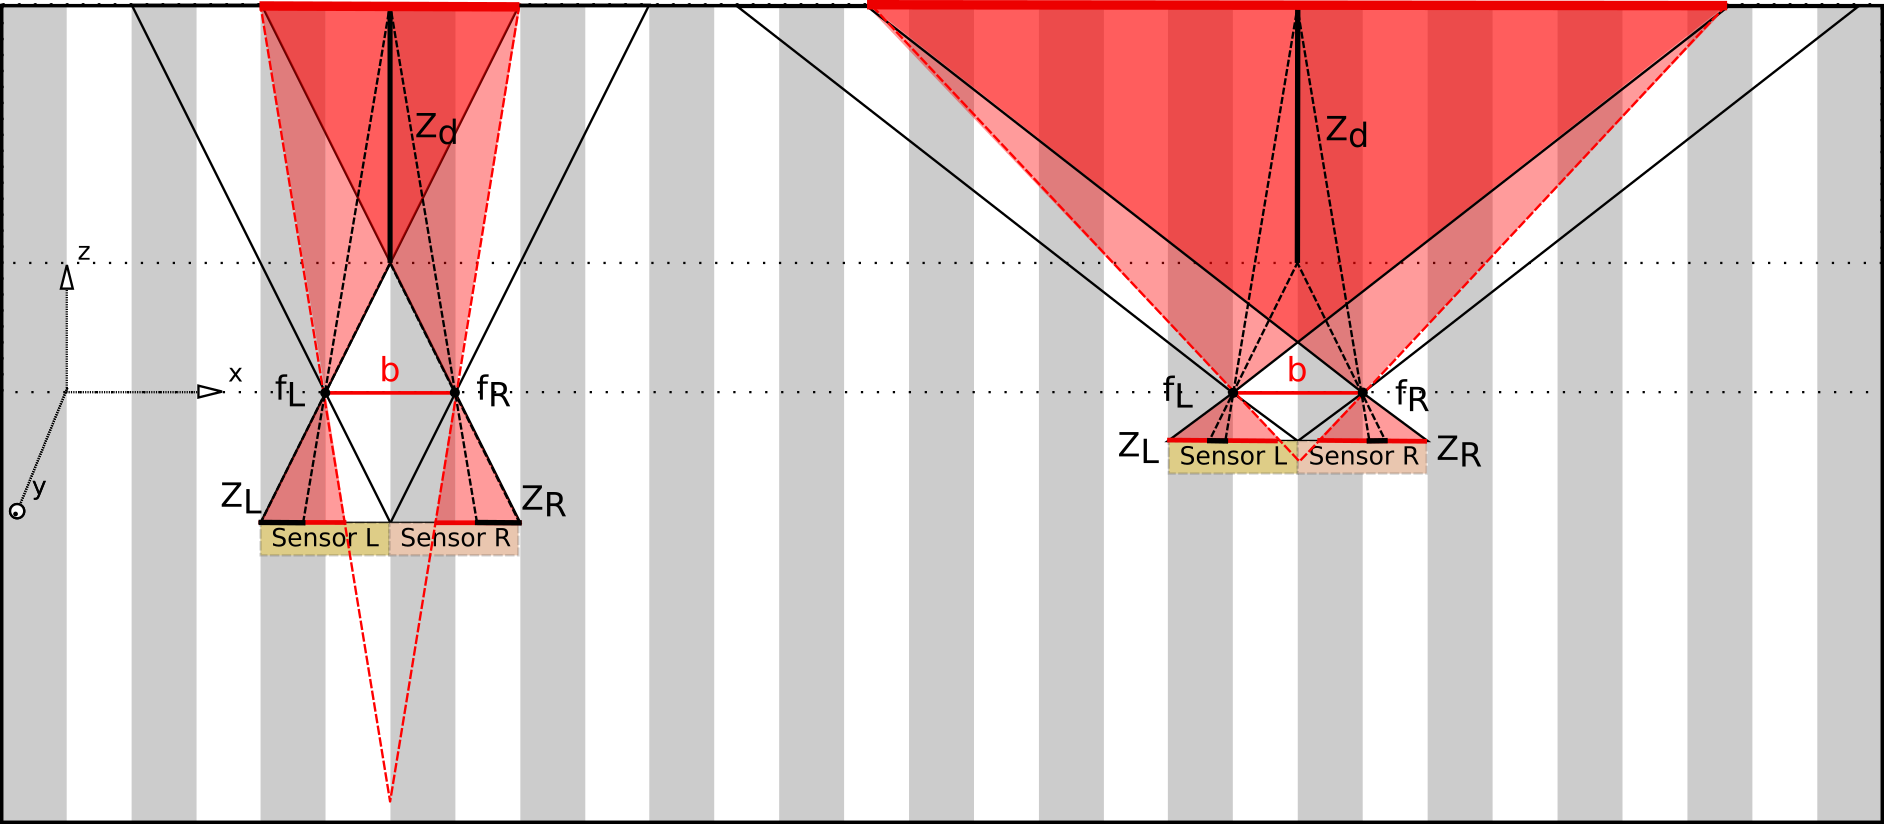
\includegraphics[width=0.80\textwidth]{./img/fundamentacao/stereo_vision_focal_variation.png}
\end{figure}

Fonte: Autor

\pagebreak

\subsection{Resolução de profundidade em função da variação da distância entre câmeras - \textit{baseline}.}

Figura \ref{fig:stereo_vision_bx_variation}

\begin{figure}[!htb]
  \centering
  \caption{Variação da \textit{baseline} ao longo do eixo x.}
  \label{fig:stereo_vision_bx_variation}
  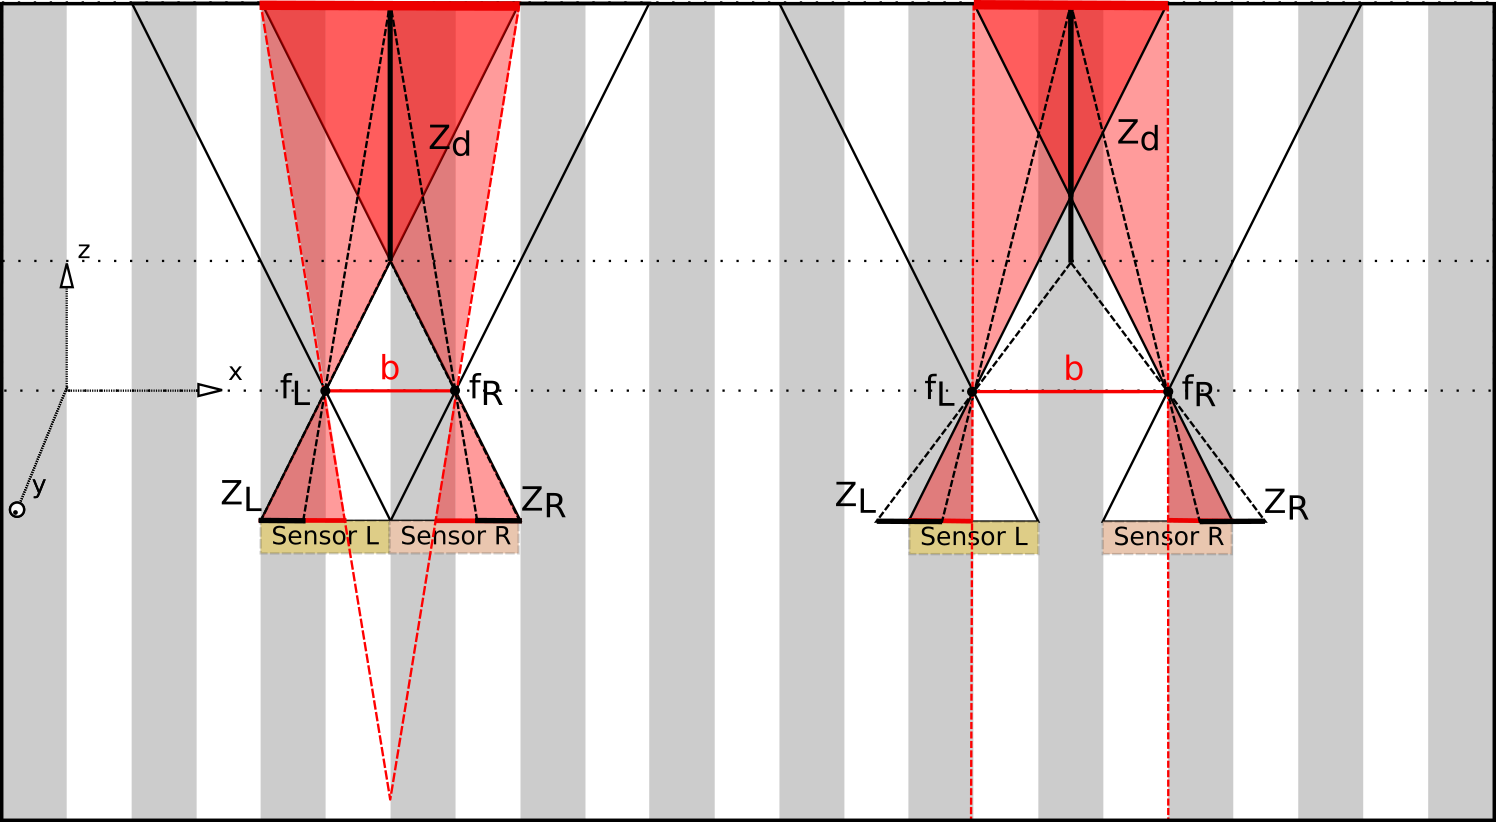
\includegraphics[width=0.80\textwidth]{./img/fundamentacao/stereo_vision_bx_variation.png}
\end{figure}

Fonte: Autor

Figura \ref{fig:stereo_vision_bz_variation}

\begin{figure}[!htb]
  \centering
  \caption{Variação da \textit{baseline} ao longo do eixo z.}
  \label{fig:stereo_vision_bz_variation}
  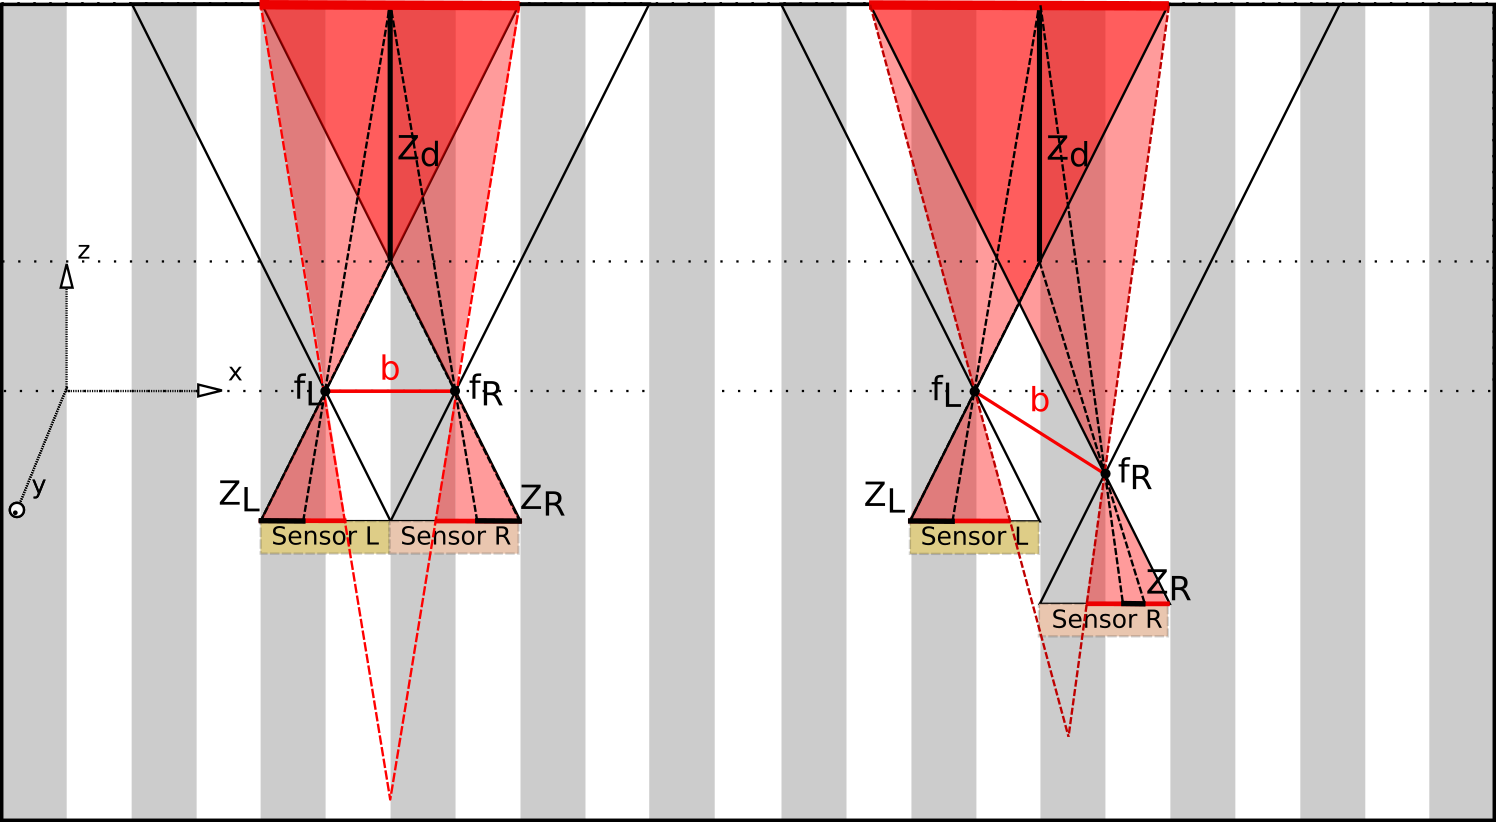
\includegraphics[width=0.80\textwidth]{./img/fundamentacao/stereo_vision_bz_variation.png}
\end{figure}

Fonte: Autor

\pagebreak

\subsection{Resolução de profundidade em função da variação do ângulo entre câmeras.}

Figura \ref{fig:stereo_vision_arc_variation}

\begin{figure}[!htb]
  \centering
  \caption{Variação do ângulo entre câmeras.}
  \label{fig:stereo_vision_arc_variation}
  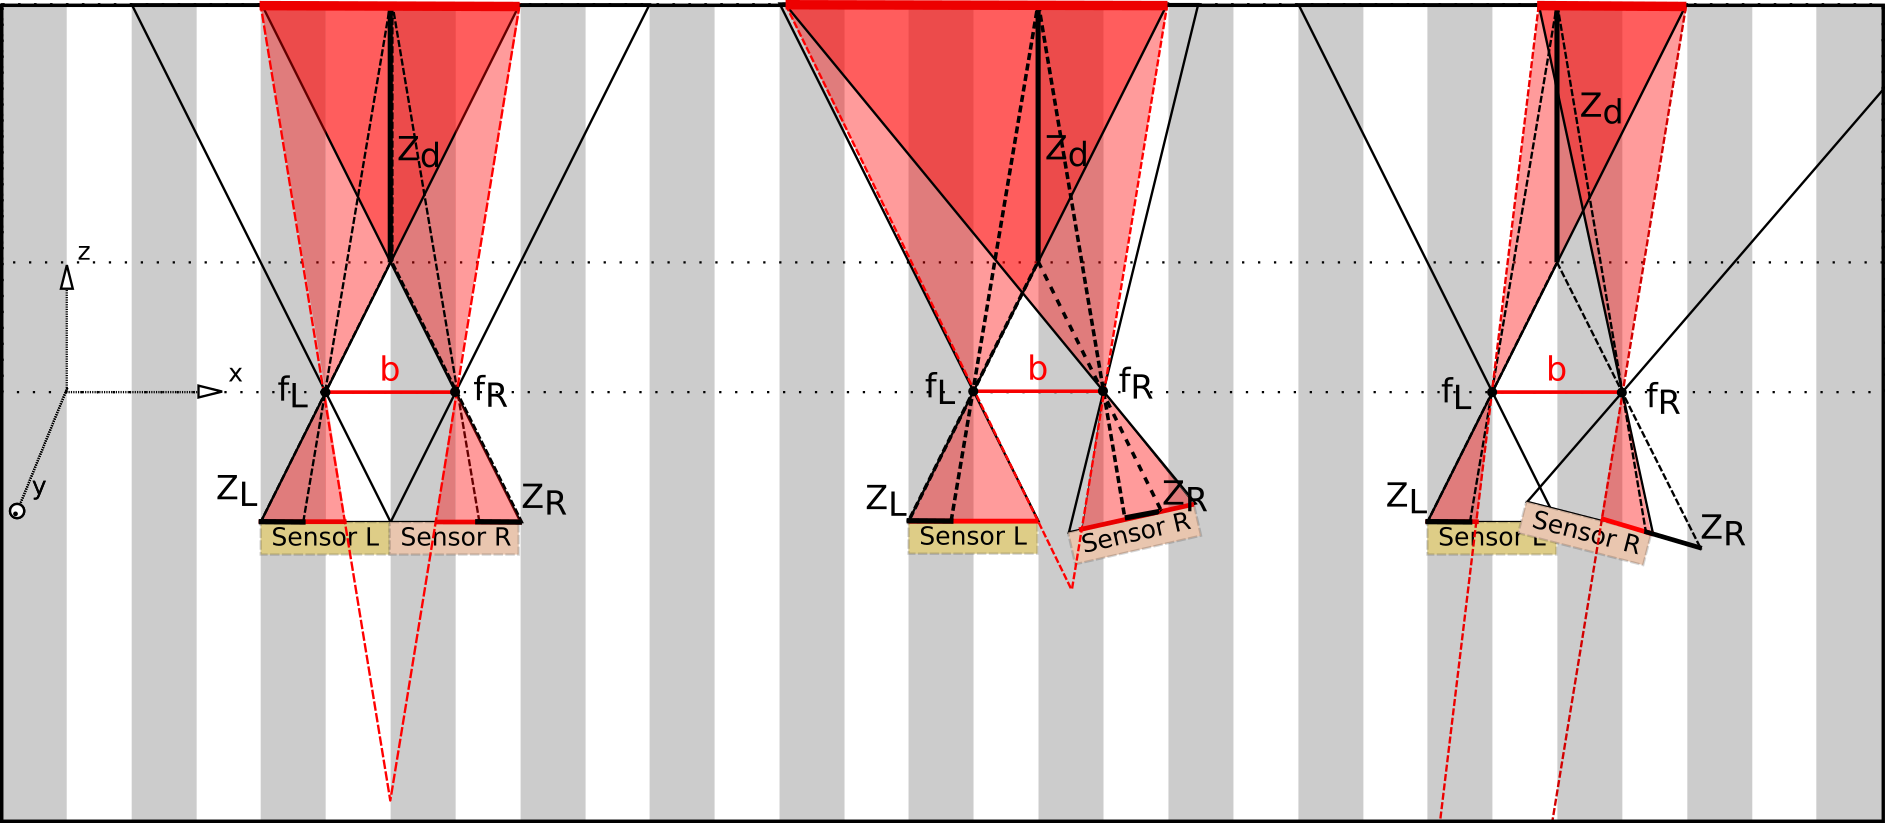
\includegraphics[width=0.80\textwidth]{./img/fundamentacao/stereo_vision_arc_variation.png}
\end{figure}
Fonte: Autor

\pagebreak

\subsection{Compensação da distância focal.}

A equação abaixo descreve a relação da resolução de profundidade $dZ_d$ com a distância total $Z$, distância focal $f$, o tamnho da\textit{baseline} $b$ e a precisão do sistema $dp_x$ \cite{Kyto2011}.

$$ dZ_d = \frac{Z^{2}}{fb}dp_x$$

Compensando a distância focal $f$ com o comprimento da \textit{baseline} $b$ é possível manter a resolução de profundidade.
É ilustrado na Figura \ref{fig:focal_dist_comp_baseline} como a ocupação dos sensores óticos $Z_L$ e $Z_R$ se mantém constante se houver uma compensação das distâncias focais $f_L$ e $f_R$ por meia da distância que separa as duas distâncias focais, $b_1$ e $b_2$.

\begin{figure}[!htb]
  \centering
  \caption{Compensação da diferença da distância focal por meio da variação da \textit{baseline}.}
  \label{fig:focal_dist_comp_baseline}
  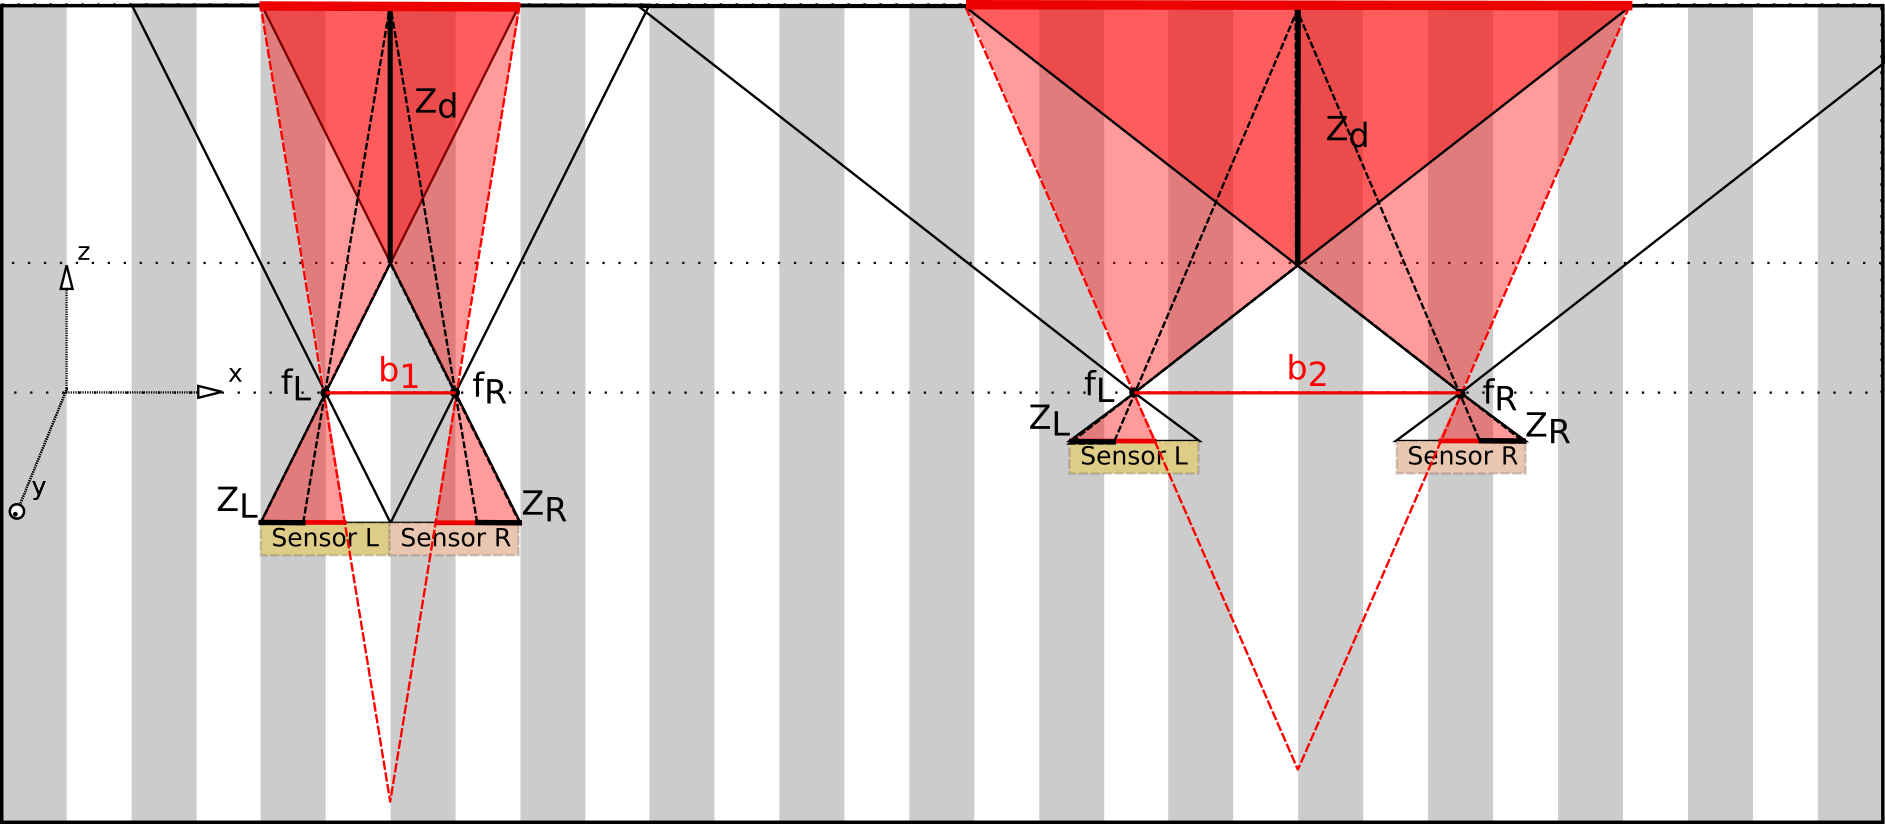
\includegraphics[width=0.95\textwidth]{./img/fundamentacao/focal_dist_comp_baseline.png}
\end{figure}

Fonte: Autor

\pagebreak

Figura \ref{fig:aberturas} 

\begin{figure}[!htb]
  \centering
  \caption{FOV - 50mm vs Logitec.}
  \label{fig:aberturas}
  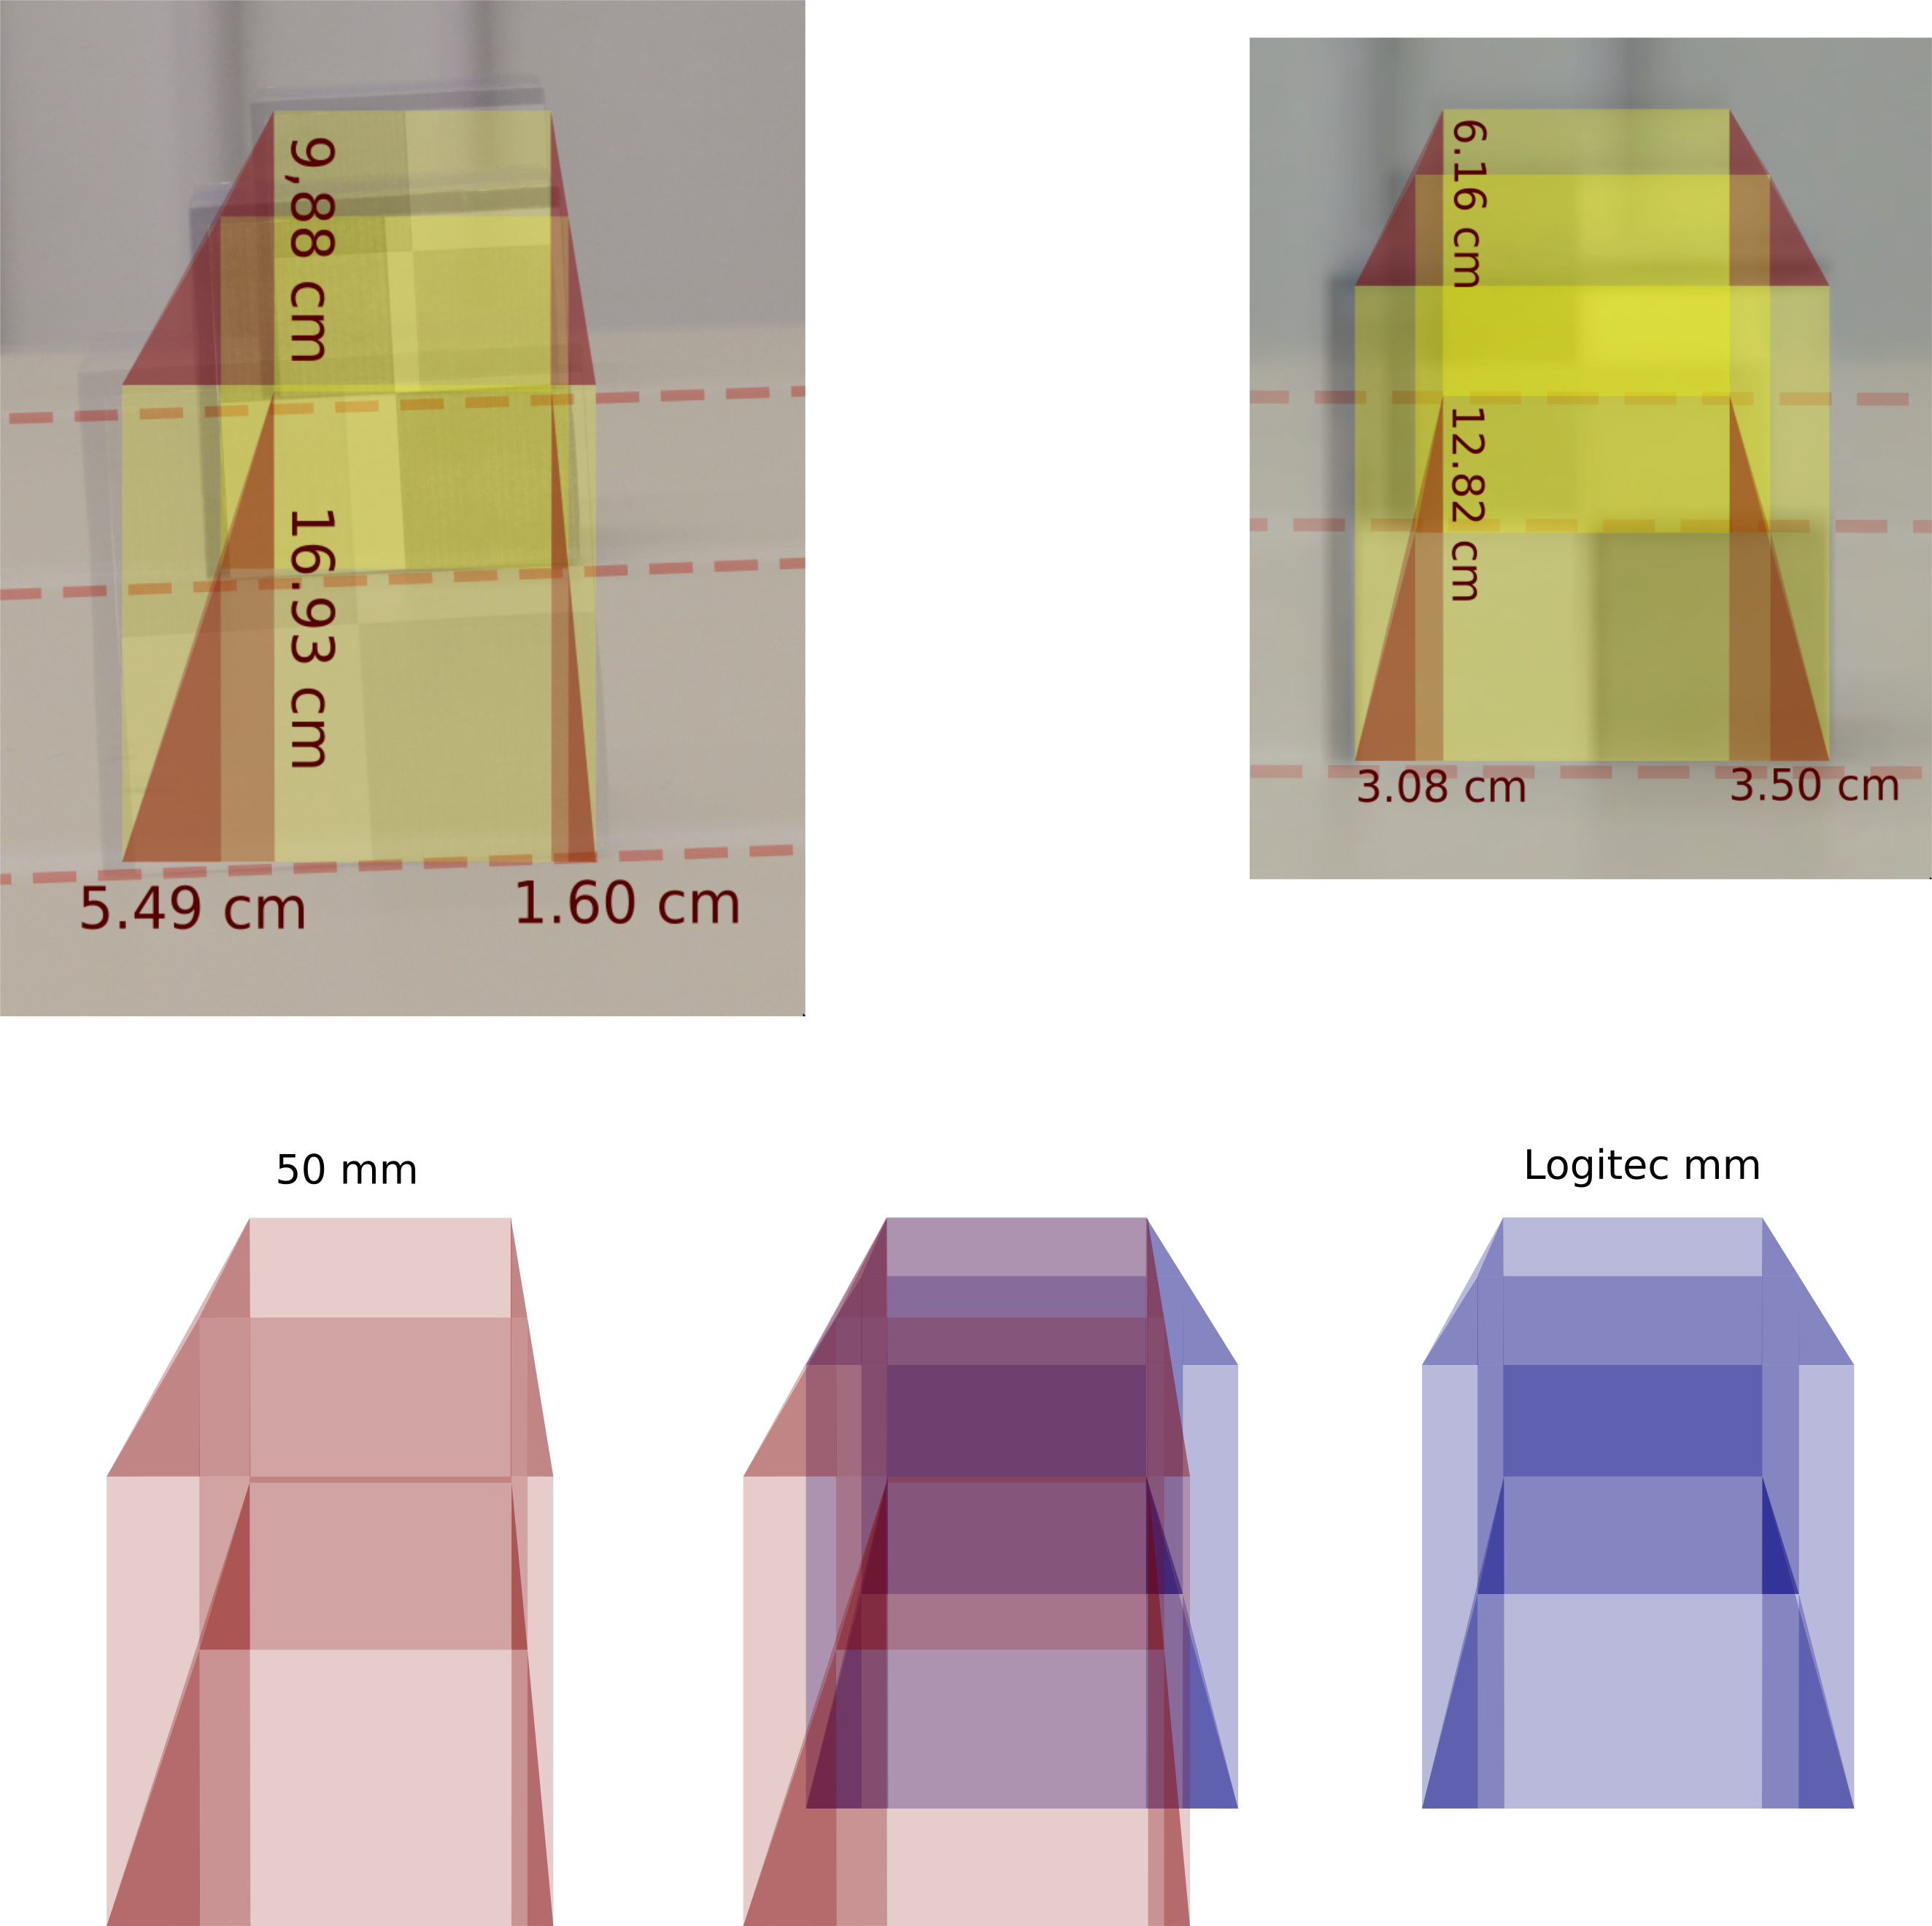
\includegraphics[width=0.80\textwidth]{./img/fundamentacao/aberturas.png}
\end{figure}

Fonte: Autor

\pagebreak

Figura \ref{fig:50m_and_logitec_equi} 

\begin{figure}[!htb]
  \centering
  \caption{Medidas da compensação da diferença da distância focal por meio da variação da \textit{baseline} utilizada no experimento.}
  \label{fig:50m_and_logitec_equi}
  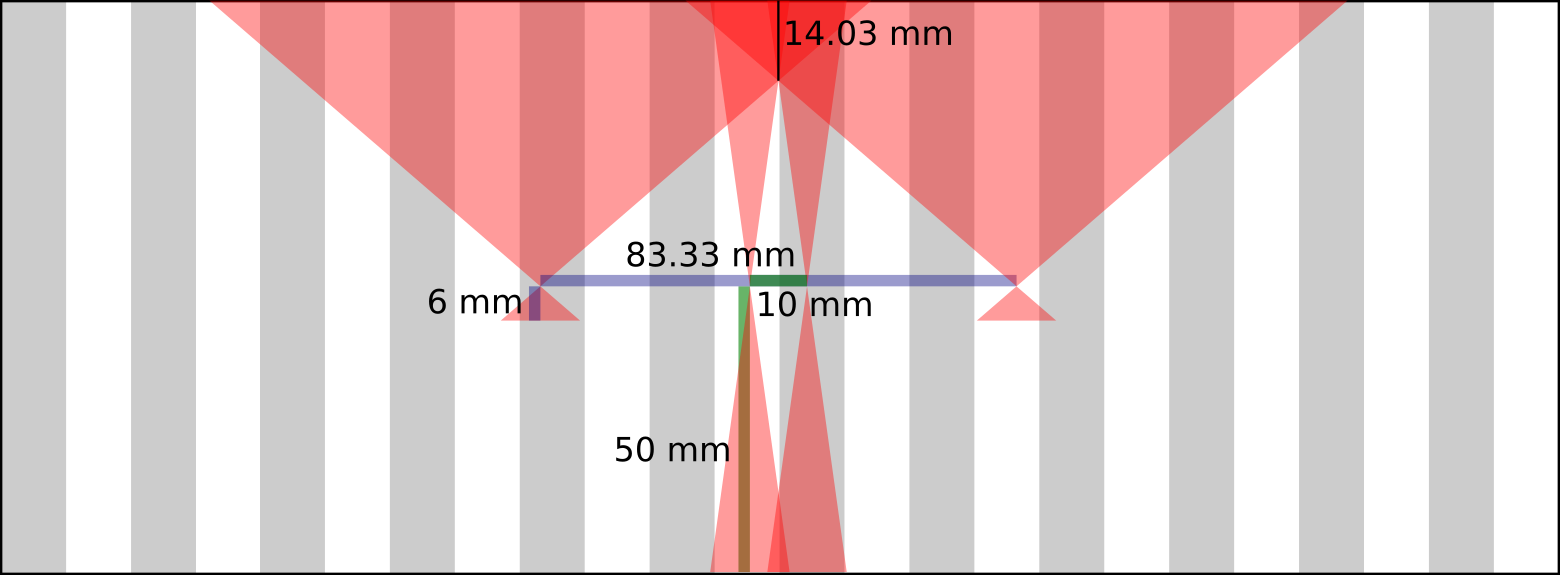
\includegraphics[width=0.80\textwidth]{./img/fundamentacao/50m_and_logitec_equi.png}
\end{figure}

Fonte: Autor

\pagebreak

% \section{Sensores de imagem}

% \pagebreak

% \subsection{Canon 500D}

% \begin{itemize}
%     \item Medidas laterais do sensor: $22.3mm \times 14.9mm = 332.3m m^{2}$ 
    
%     \item Medida diagonal do sensor: $26.82mm$.

%     \item Fator de Corte: $1.61$.
    
%     \item Espaçamento entre pixel: $4.68\mu m$.
    
%     \item Área do pixel: $21.9\mu m^{2}$.
    
%     \item Densidade de pixel: $4.56 Mega Pixel/cm^{2}$. 
% \end{itemize}

% \pagebreak

% \ref{fig:focal_dist_test_1} 

% \begin{figure}[!htb]
%   \centering
%   \caption{Teste de distância focal.}
%   \label{fig:focal_dist_test_1}
%   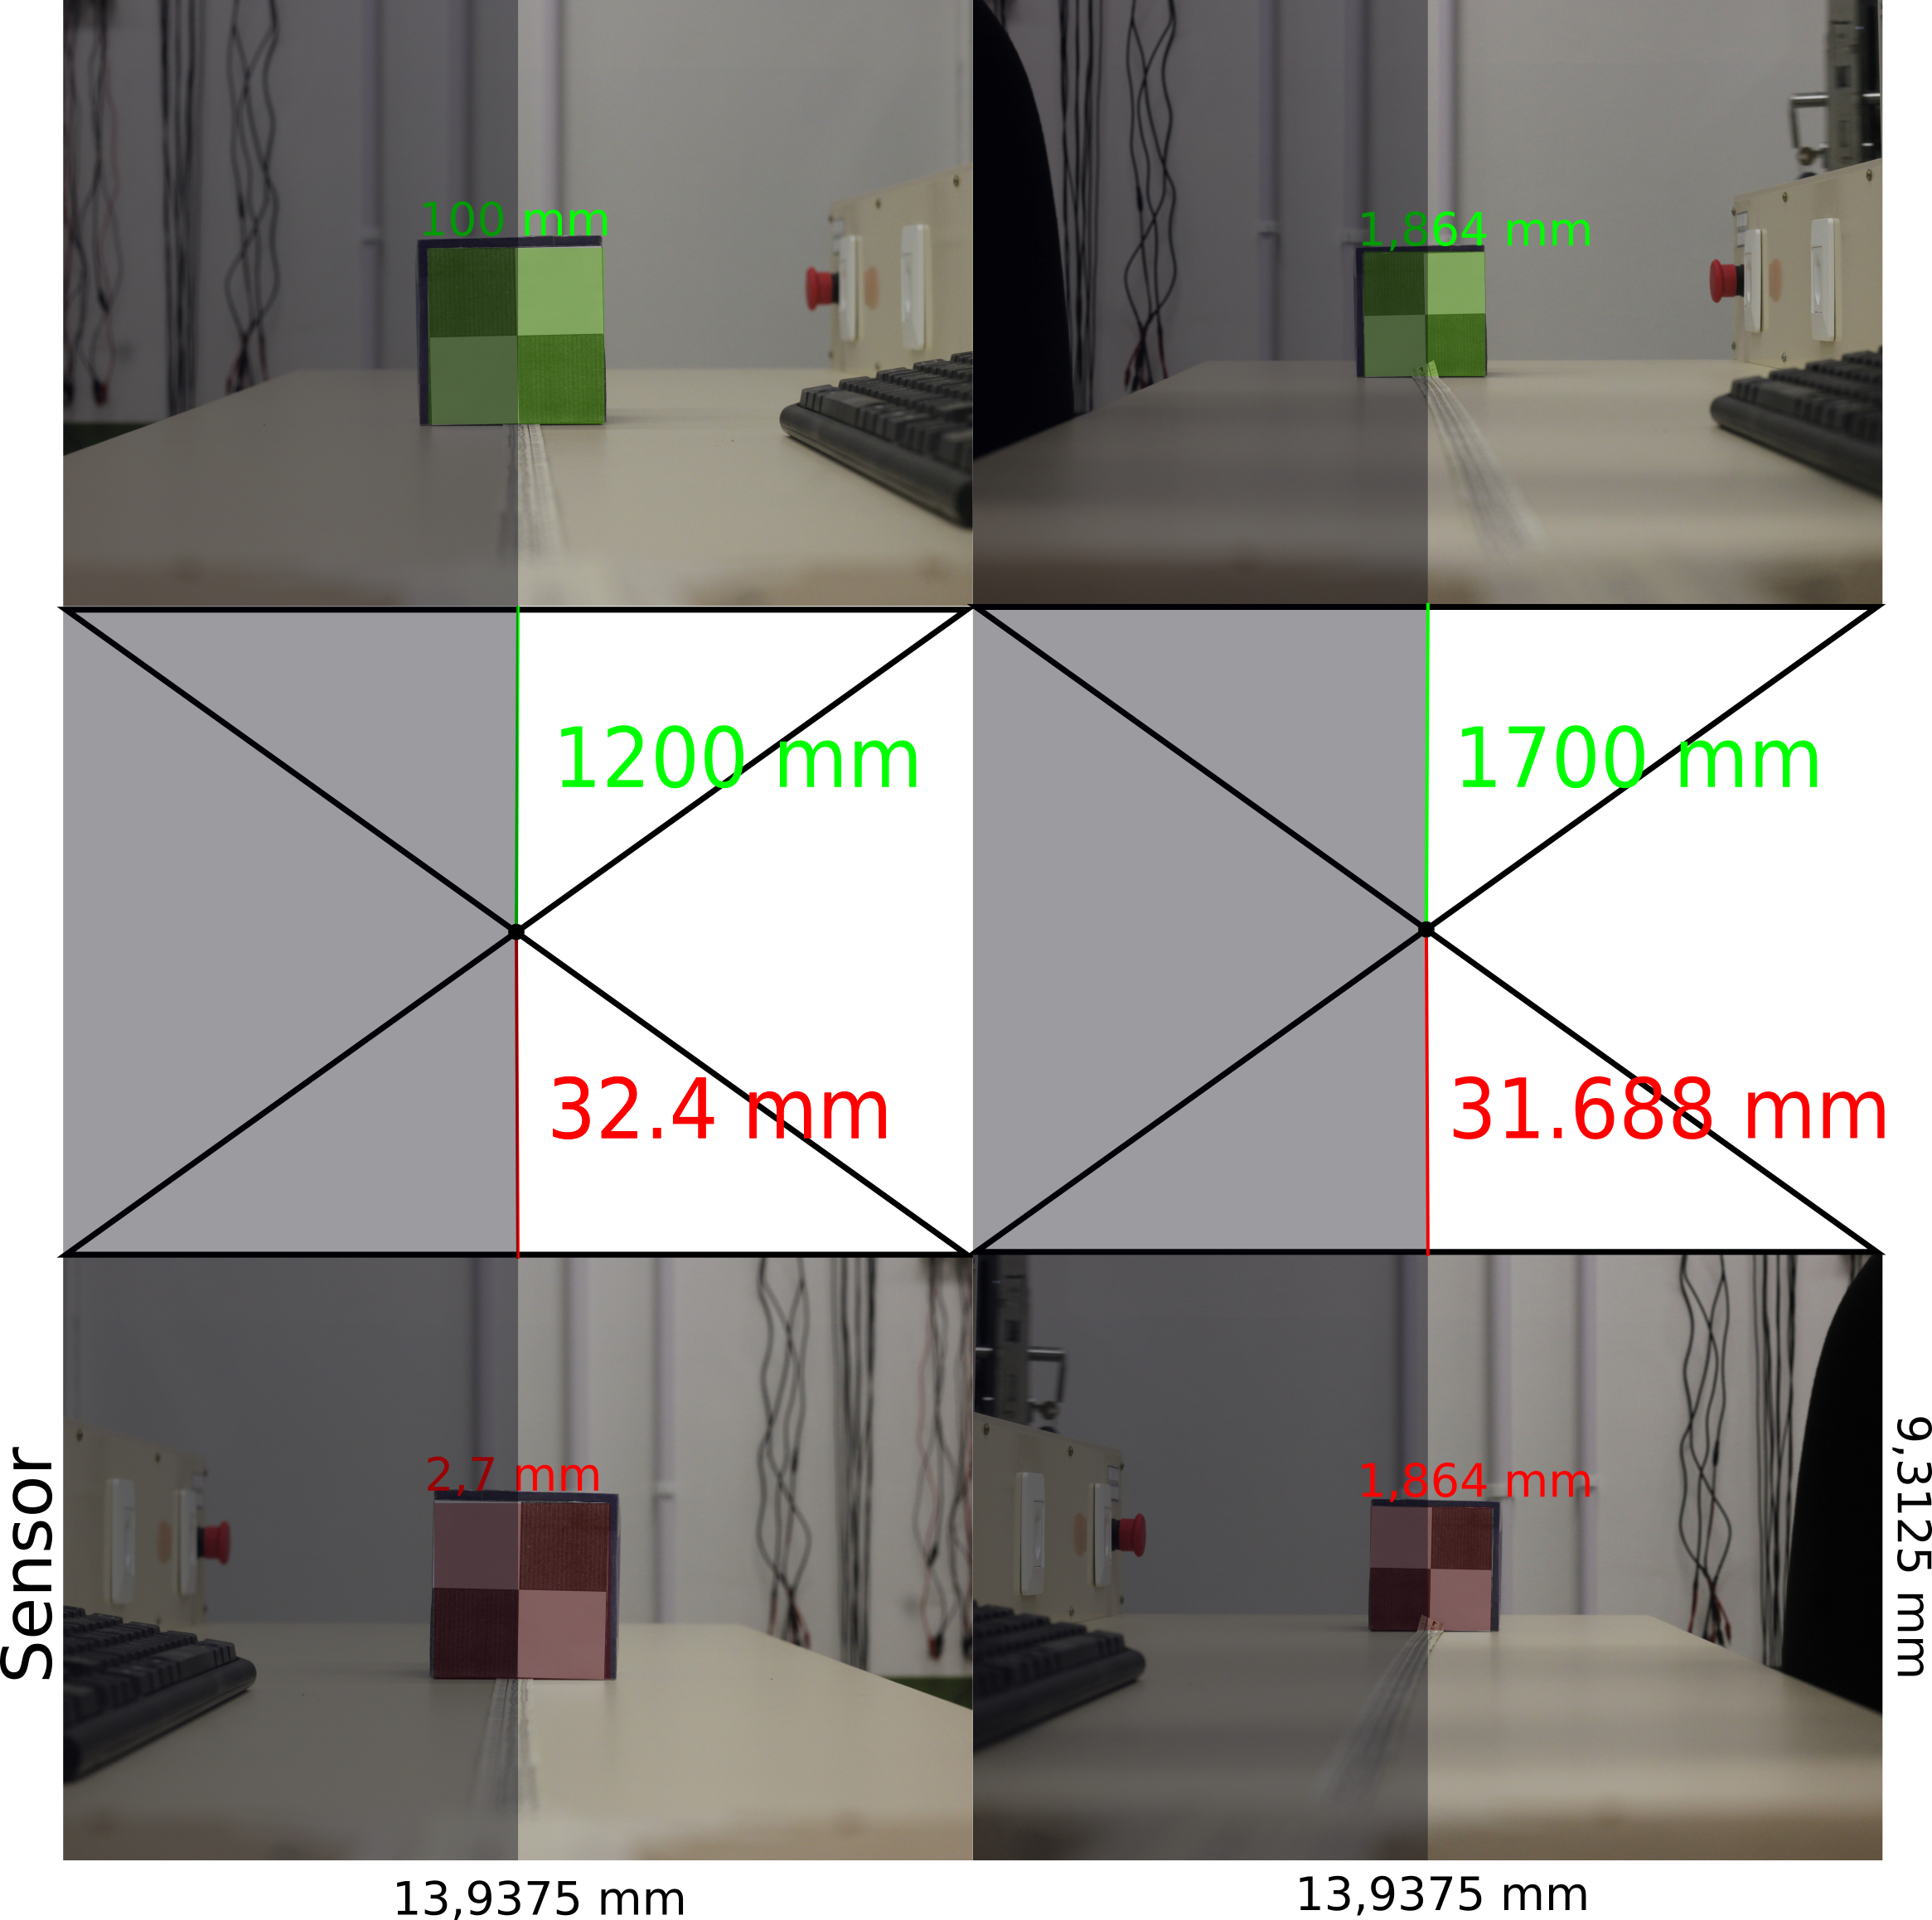
\includegraphics[width=0.80\textwidth]{./img/focal_dist_test_1.png}
% \end{figure}
% Fonte: Autor

% \pagebreak


% \subsection{Logitec}

% \pagebreak

% \subsection{Calibração das Câmeras}

% \begin{figure}[!htb]
%   \centering
%   \caption{Representação Geométrica da Câmera.}
%   \label{fig:cammat_img}
%   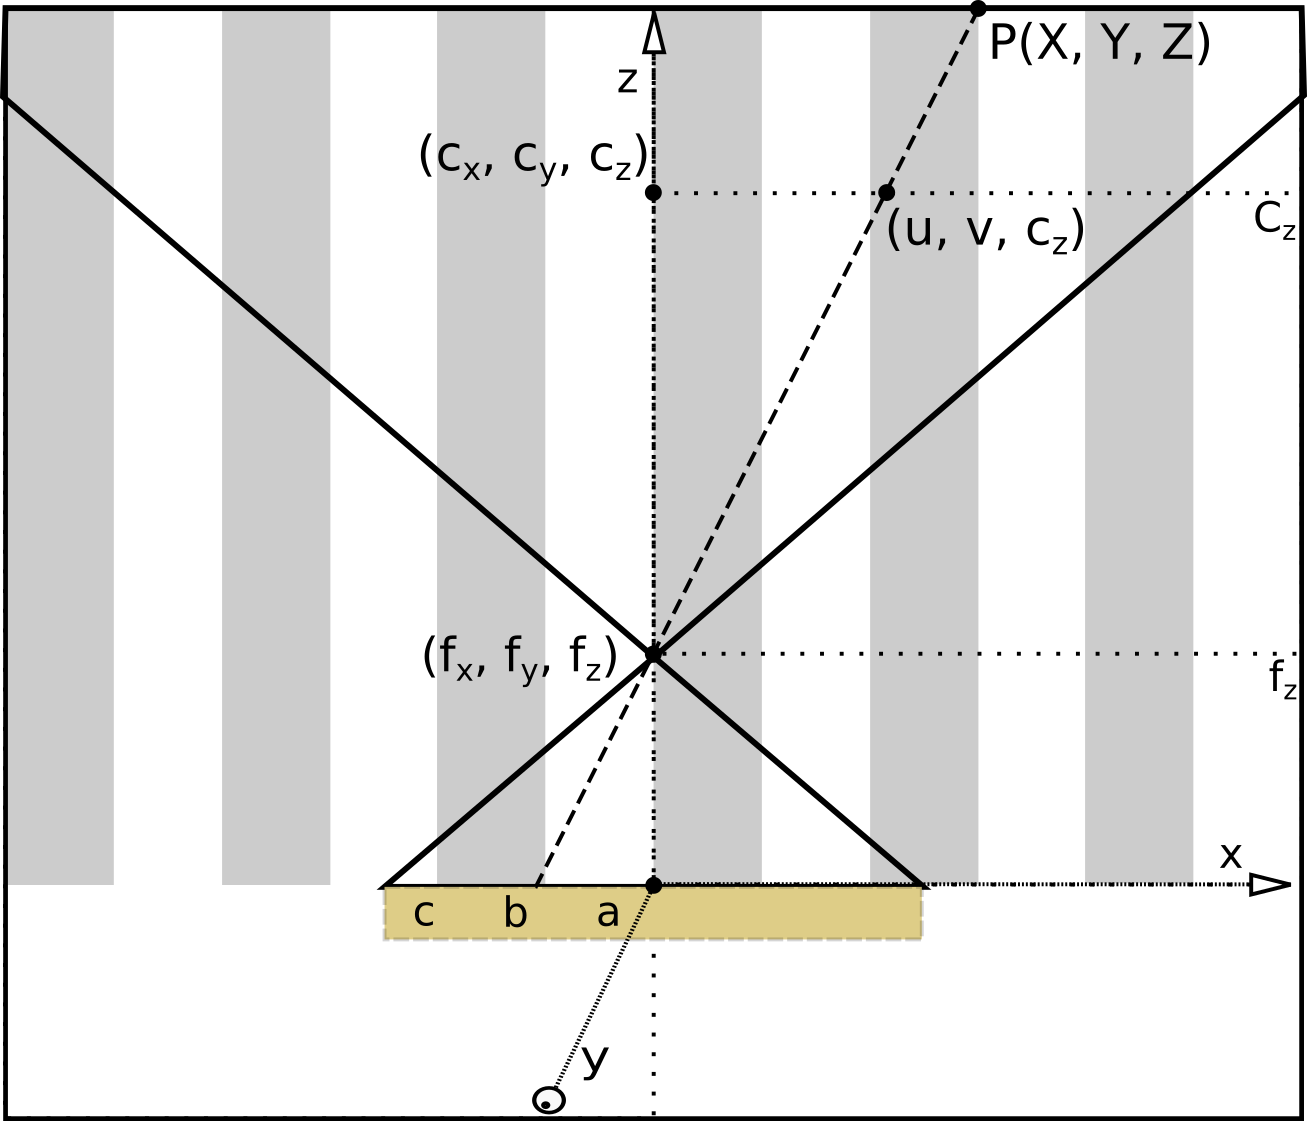
\includegraphics[width=0.80\textwidth]{./img/cammat_img.png}
% \end{figure}
% Fonte: Autor

% \pagebreak

\section{Acionamento de motor DC}

\subsection{\textit{Tri Motor Shield}}

\cite{borges2019}

\begin{figure}[!htb]
  \centering
  \caption{Tri Motor Shield acoplado ao módulo Arduino Uno.}
  \label{fig:TriMotorShield}
  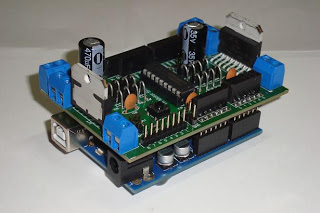
\includegraphics[width=0.60\textwidth]{./img/fundamentacao/TriMotorShield.jpg}
\end{figure}
Fonte: \textit{Borges \textit{Corporation}}

\pagebreak

\subsection{Ponte H L298N}

Como apresentado na Figura \ref{fig:L298N_block_diagram}, esse componente é composto de dois \textit{drivers} de corrente contínua de topologia Ponte H. Seu acionamento pode ser efetuado com padrão de nível lógico \textit{TTL}. A tensão máxima de operação é $50V$ e a corrente contínua máxima suportada é $2A$ \cite{stmicroelectronics2000}.

\begin{figure}[!htb]
  \centering
  \caption{Esquemático do L298N.}
  \label{fig:L298N_block_diagram}
  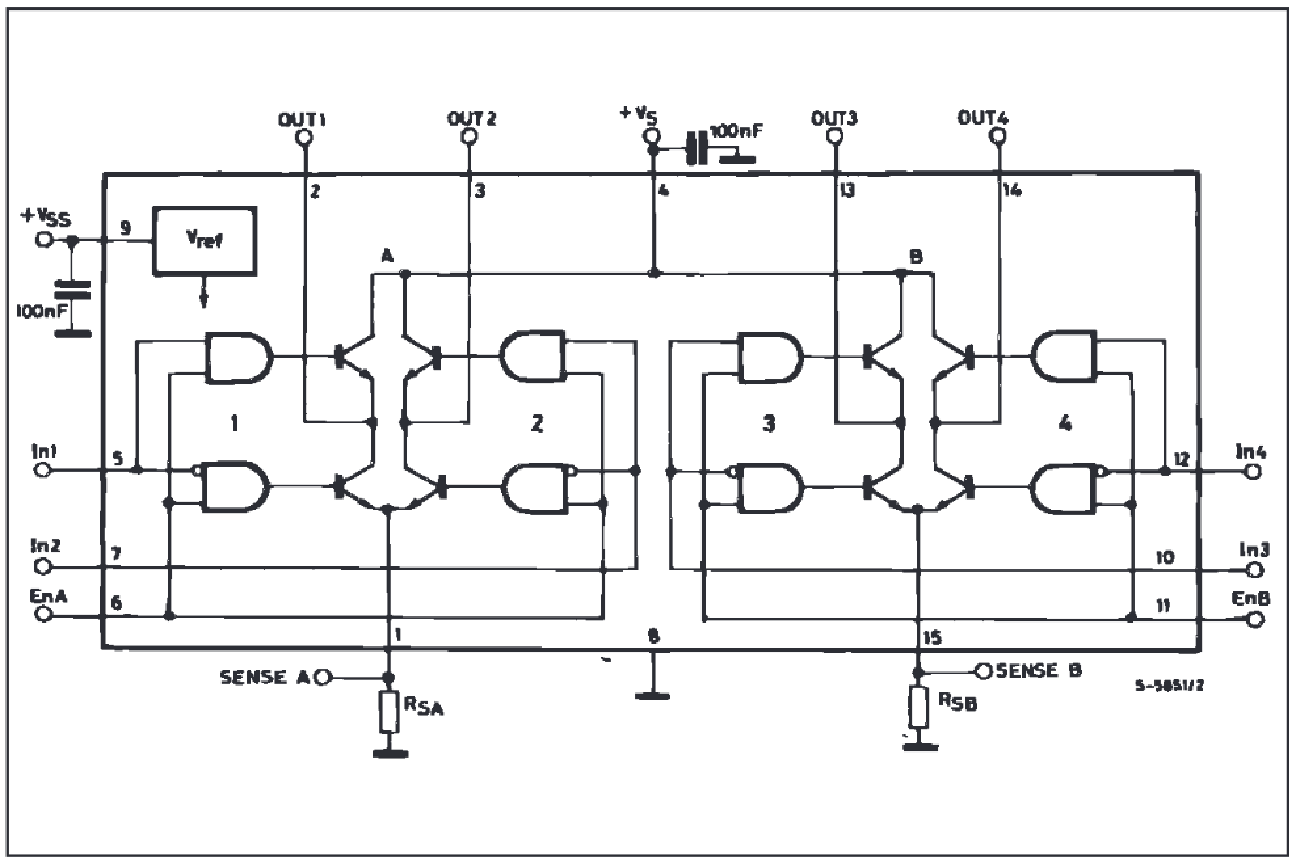
\includegraphics[width=0.95\textwidth]{./img/fundamentacao/L298N_block_diagram.png}
\end{figure}
Fonte: \textit{STMicroelectronics}


\chapter{Concepções}

\section{Concepção da plataforma de prototipagem}

Sistemas com \textit{linux} embarcado possibilitam o uso da biblioteca OpenCV \cite{Suryatali2015}. Além disso facilitam as práticas de prototipagem. Isso pois para atualizar um algorítimo específico, não há a necessidade de desligar o sistema para regravar o \textit{firmware}.
Porém processadores de baixo custo que rodam \textit{linux} embarcado, como os presentes nas placas \textit{Raspberry Pi}, possuem um tempo de resposta impreciso para acionar o GPIO. Logo um processador de tempo real é necessário para geração dos sinais PWM que irão controlar a potência fornecida aos motores. Por meio de uma comunicação serial processador rodando \textit{linux} embarcado envia o valor de potência para o processador de tempo real. Esse deve modular o valor de potência em valor de largura de pulso para acionamento do motores, como indicado na Figura \ref{fig:mapa_sys}. 

\begin{figure}[!htb]
  \centering
  \caption{Mapa do Sistema.}
  \label{fig:mapa_sys}
  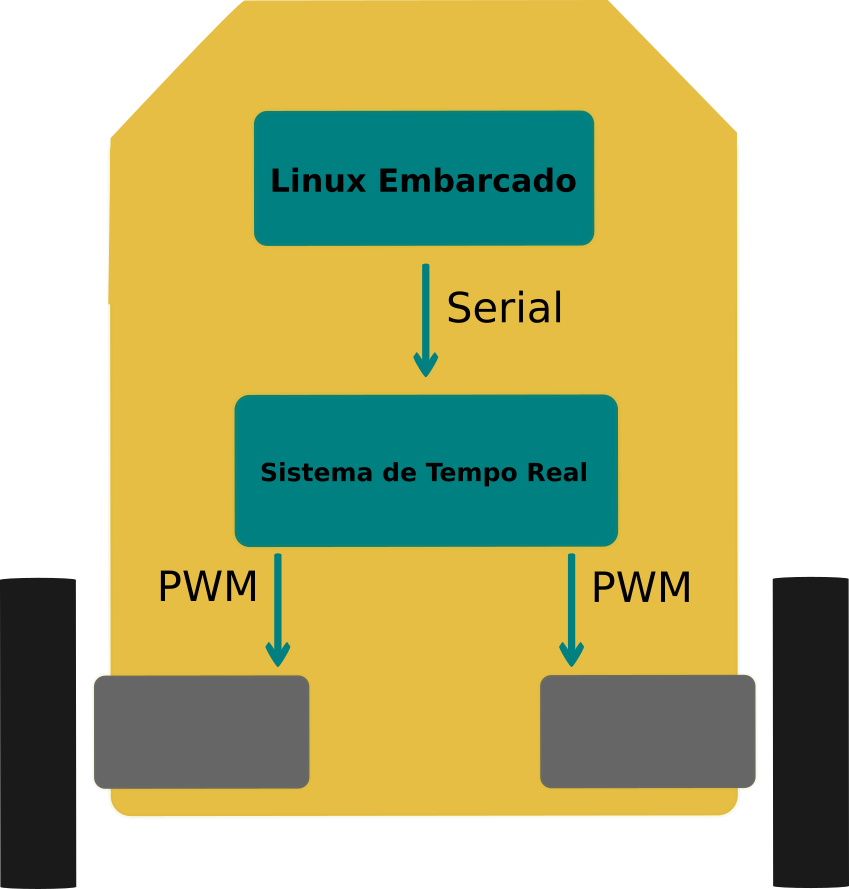
\includegraphics[width=0.7\textwidth]{./img/concepcao/mapa_sys.png}
\end{figure}
Fonte: \textit{Autor}

\pagebreak

Com um acelerômetro de baixo custo se torna possível a implementação de uma interface de controle. 
Considerando que o acelerômetro seja capaz de medir valores constantes de aceleração nos três eixos, é possível usar a direção da gravidade da terra como referencial para medir a inclinação do mesmo. 
Logo é possível a implementação de um manche, pois com o acelerômetro acoplado no mesmo é possível identificar quando esse é inclinado. A Figura \ref{fig:controle_diferencial} ilustra a situação onde o valor da componente y da gravidade medidos pelo acelerômetro é associado ao valor da diferença de potência aplicada entre os motores. Assim se tem associado o raio da curva exercida á inclinação do acelerômetro.

\begin{figure}[!htb]
  \centering
  \caption{Controle de Curva.}
  \label{fig:controle_diferencial}
  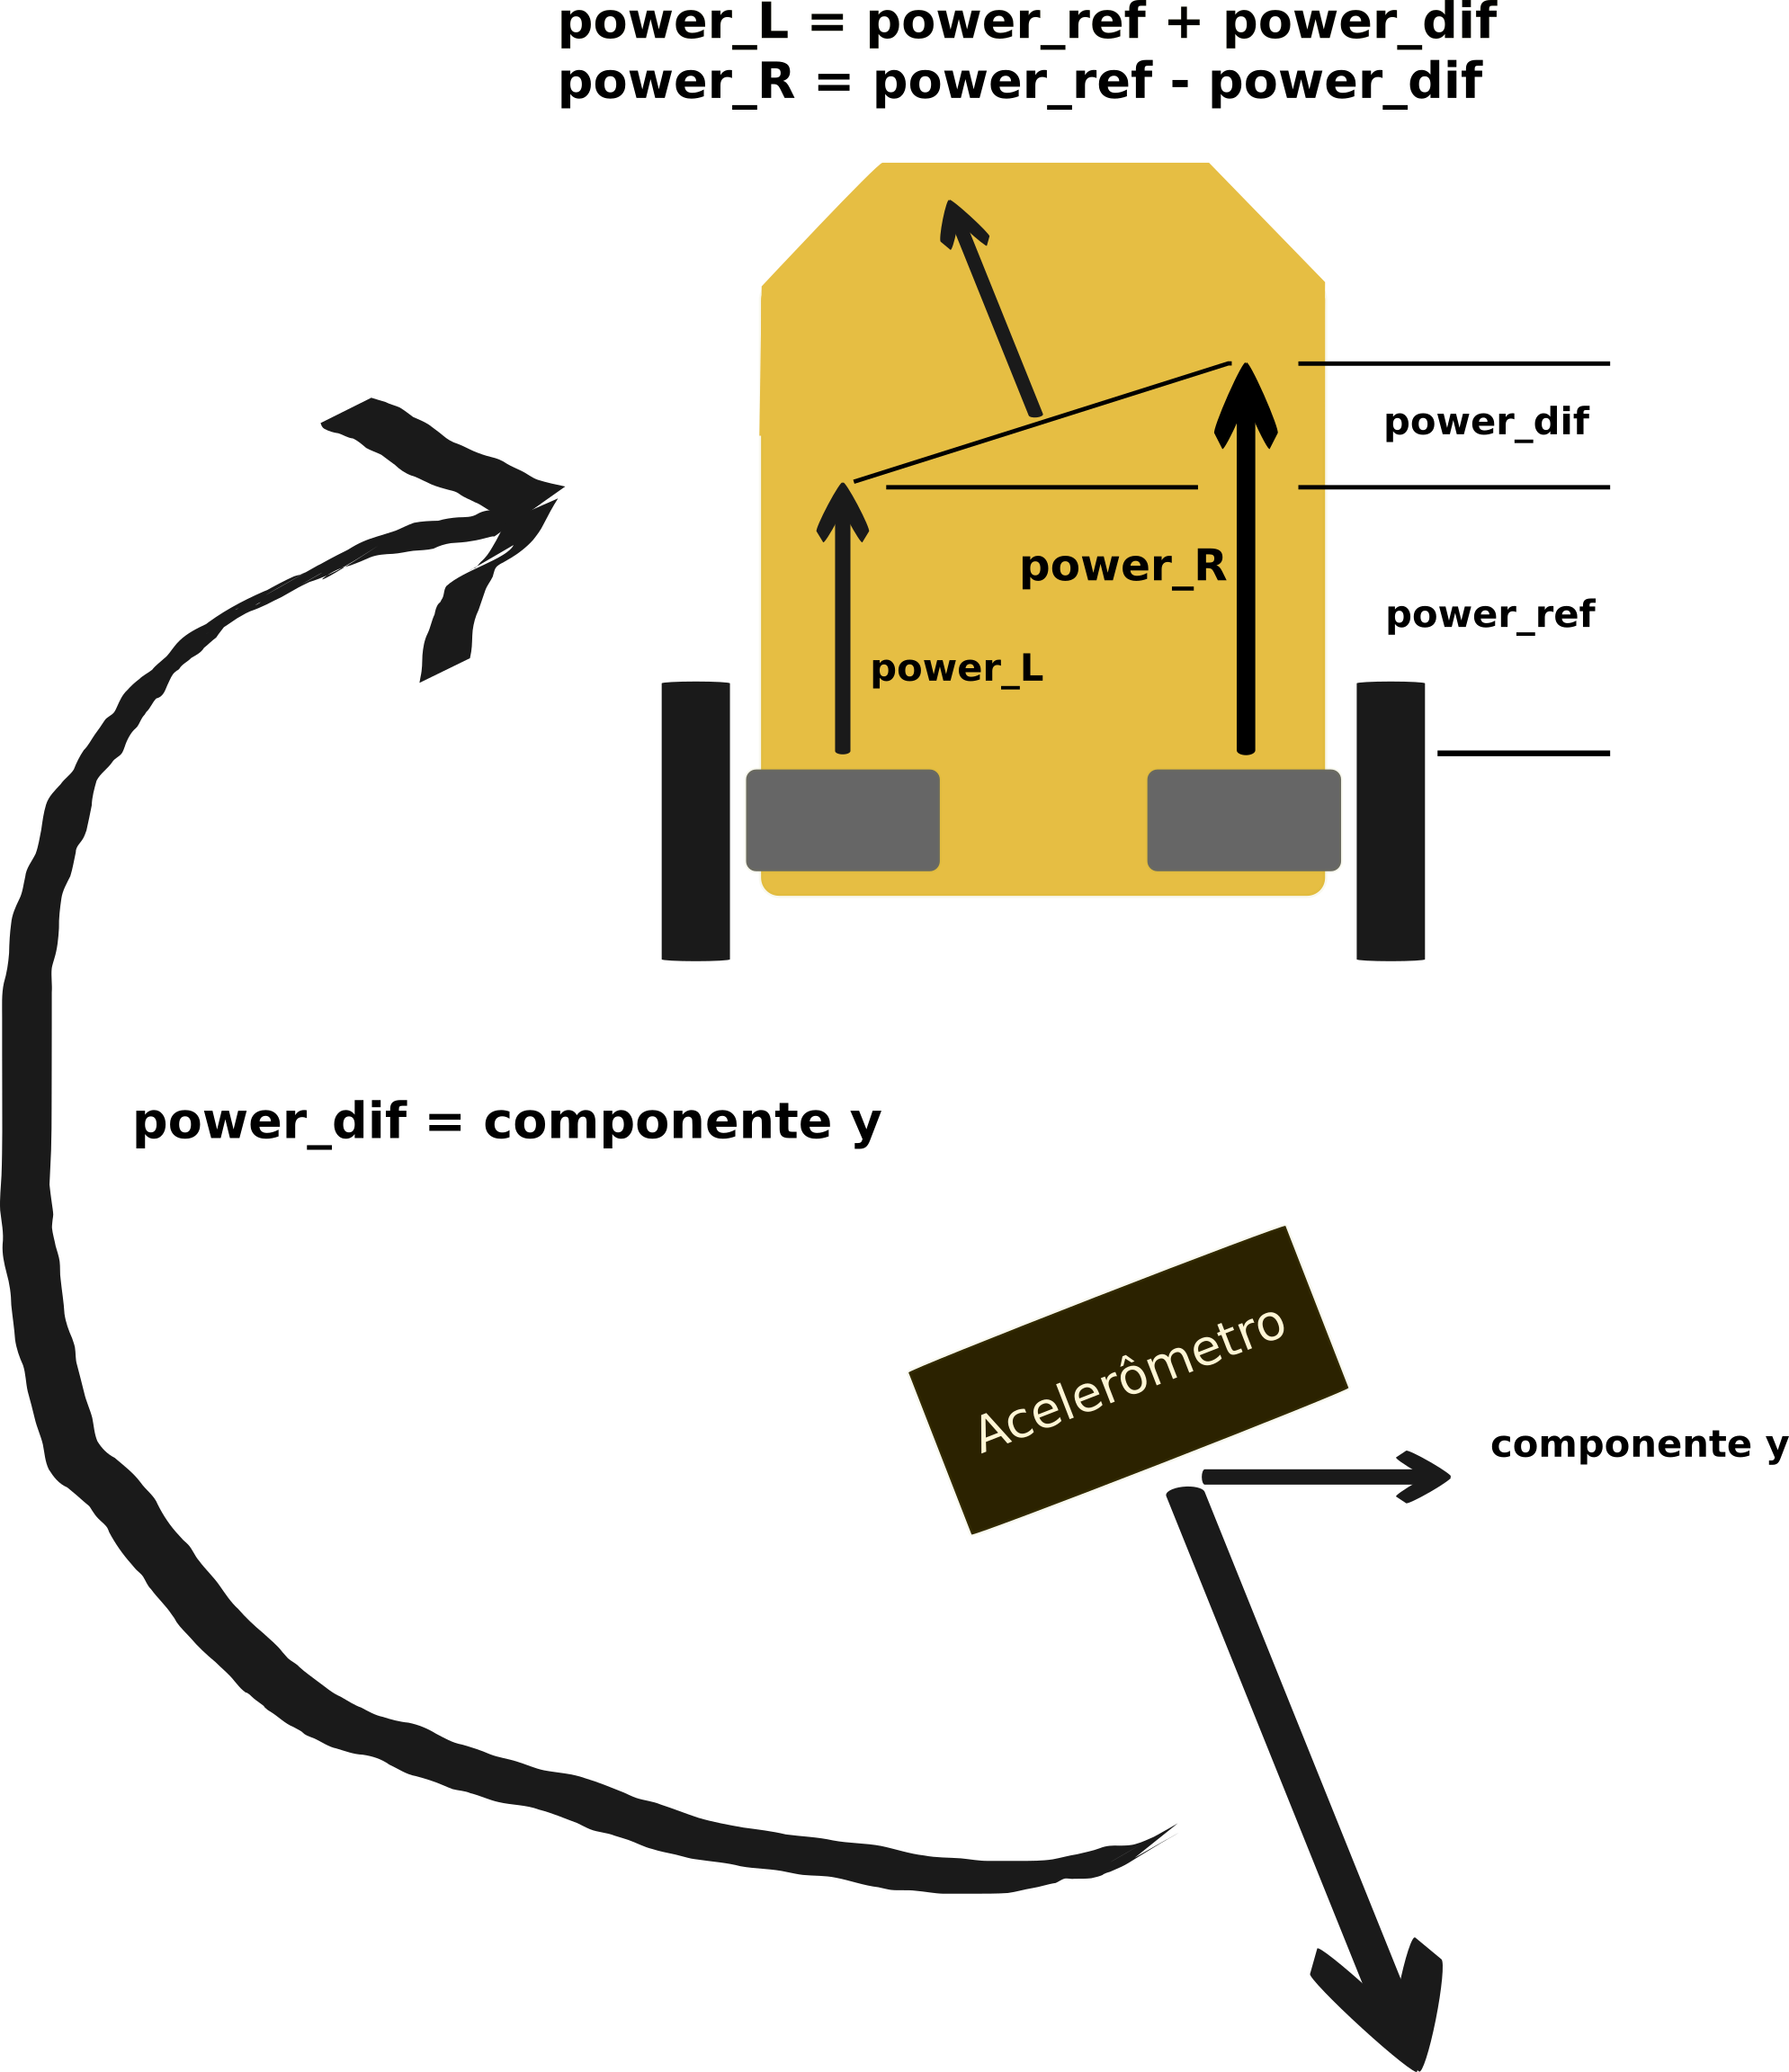
\includegraphics[width=0.80\textwidth]{./img/concepcao/controle_diferencial.png}
\end{figure}
Fonte: \textit{Autor}

\pagebreak

A unidade de controle se comunica com uma interface de controle como apresentado na Figura \ref{fig:controle_para_atuador}.

\begin{figure}[!htb]
  \centering
  \caption{Interface de controle.}
  \label{fig:controle_para_atuador}
  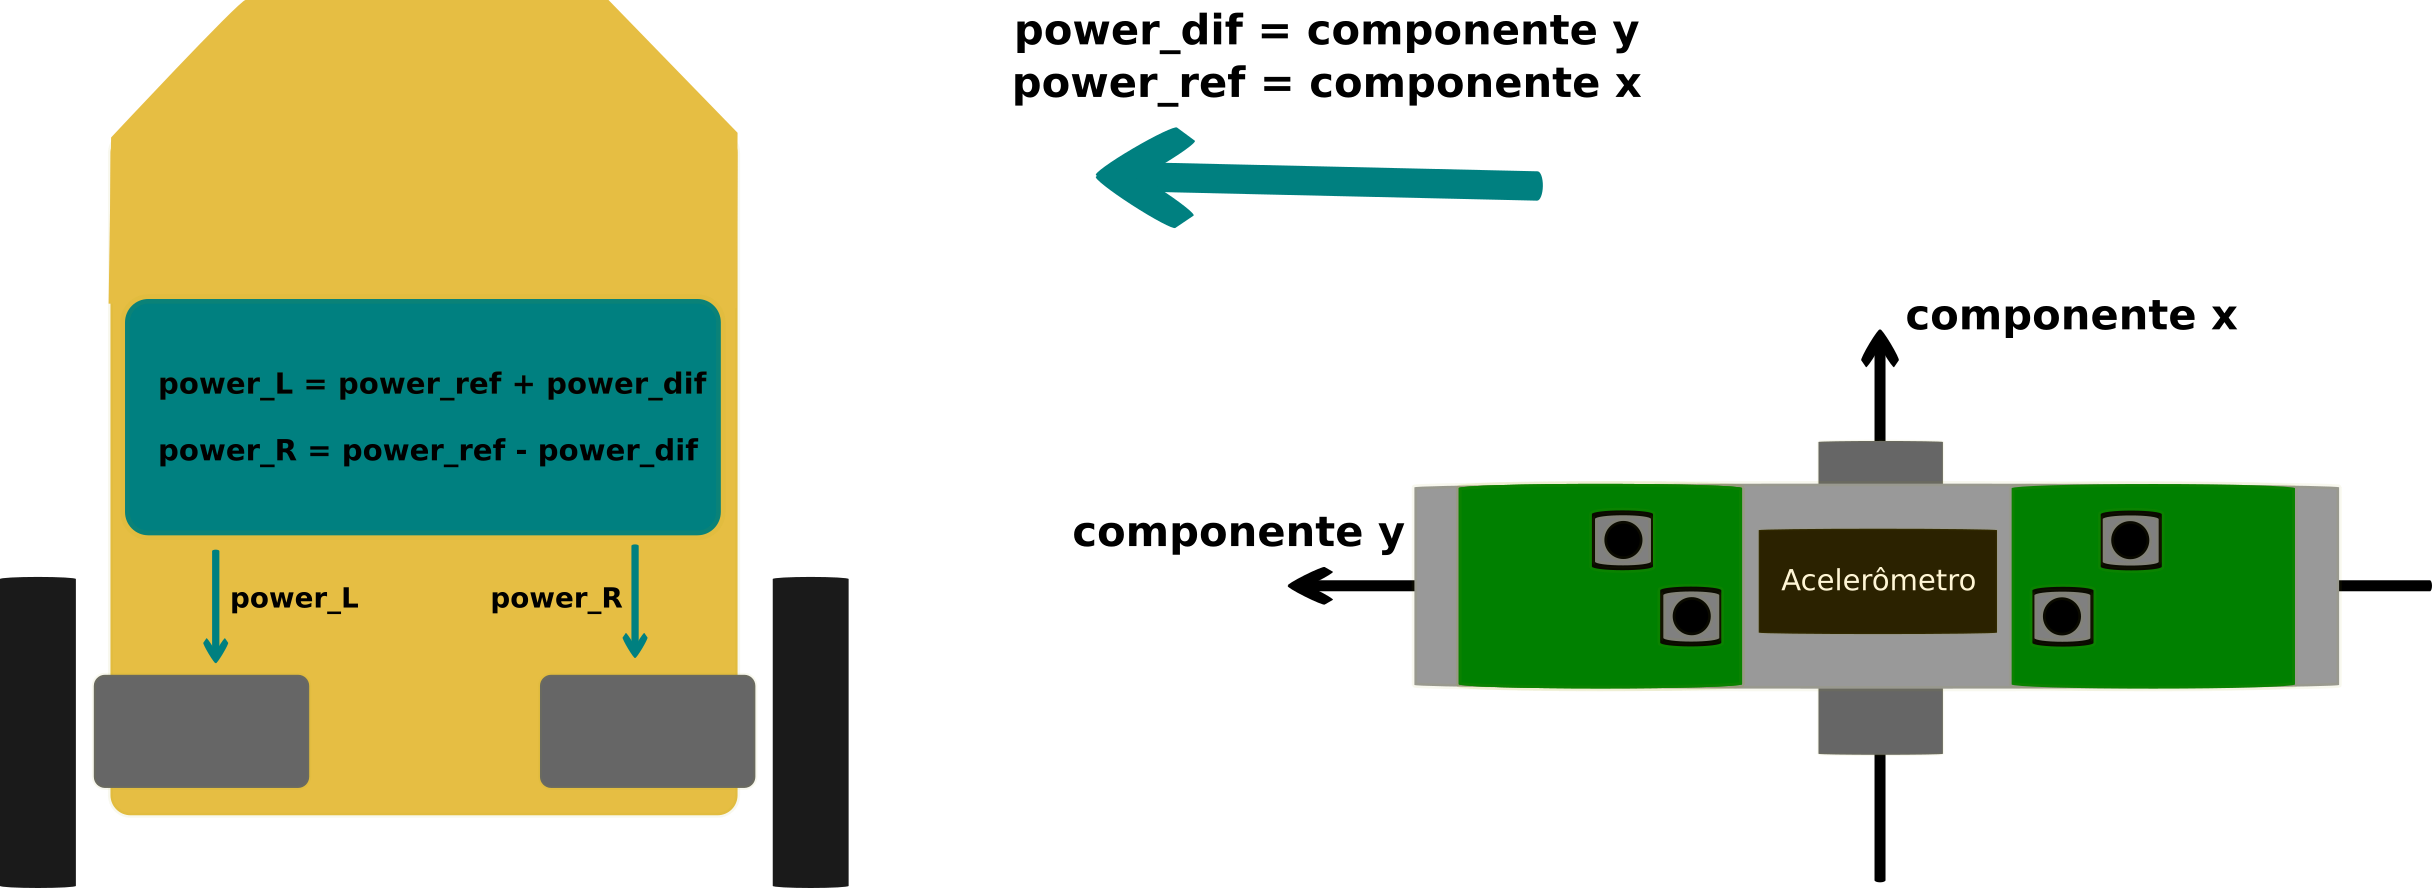
\includegraphics[width=0.95\textwidth]{./img/concepcao/controle_para_atuador.png}
\end{figure}
Fonte: \textit{Autor}

Uma vez podendo controlar de forma independente a potência que é aplicada em cada motor, é possível exercer curvas de raios diferentes. 
Na Figura \ref{fig:angulo_dif_power} é exemplificado o caso onde a diferença da potência aplicada entre os motores do Carro A é menor que no Carro B.

\begin{figure}[!htb]
  \centering
  \caption{Diferença de potência aplicada aos motores.}
  \label{fig:angulo_dif_power}
  \includegraphics[width=0.7\textwidth]{./img/concepcao/angulo_dif_power.png}
\end{figure}
Fonte: \textit{Autor}

\pagebreak

A interface de controle pode ser implementada como apresentado na Figura \ref{fig:controle_acelerometro}. Um acelerômetro de três eixos é capaz de decompor o vetor de aceleração em duas componentes independentes. Dessa forma, além da componente y associada ao controle de curva, é possível associar a componente x ao controle de velocidade. Dessa forma, inclinando o manche na direção da componente x é possível controlar a potência que é aplicada em ambos os motores. Assim como inclinando o o manche na direção y é possível controlar a diferença de potência que é aplicada entre os motores. 

\begin{figure}[!htb]
  \centering
  \caption{Interface de Controle.}
  \label{fig:controle_acelerometro}
  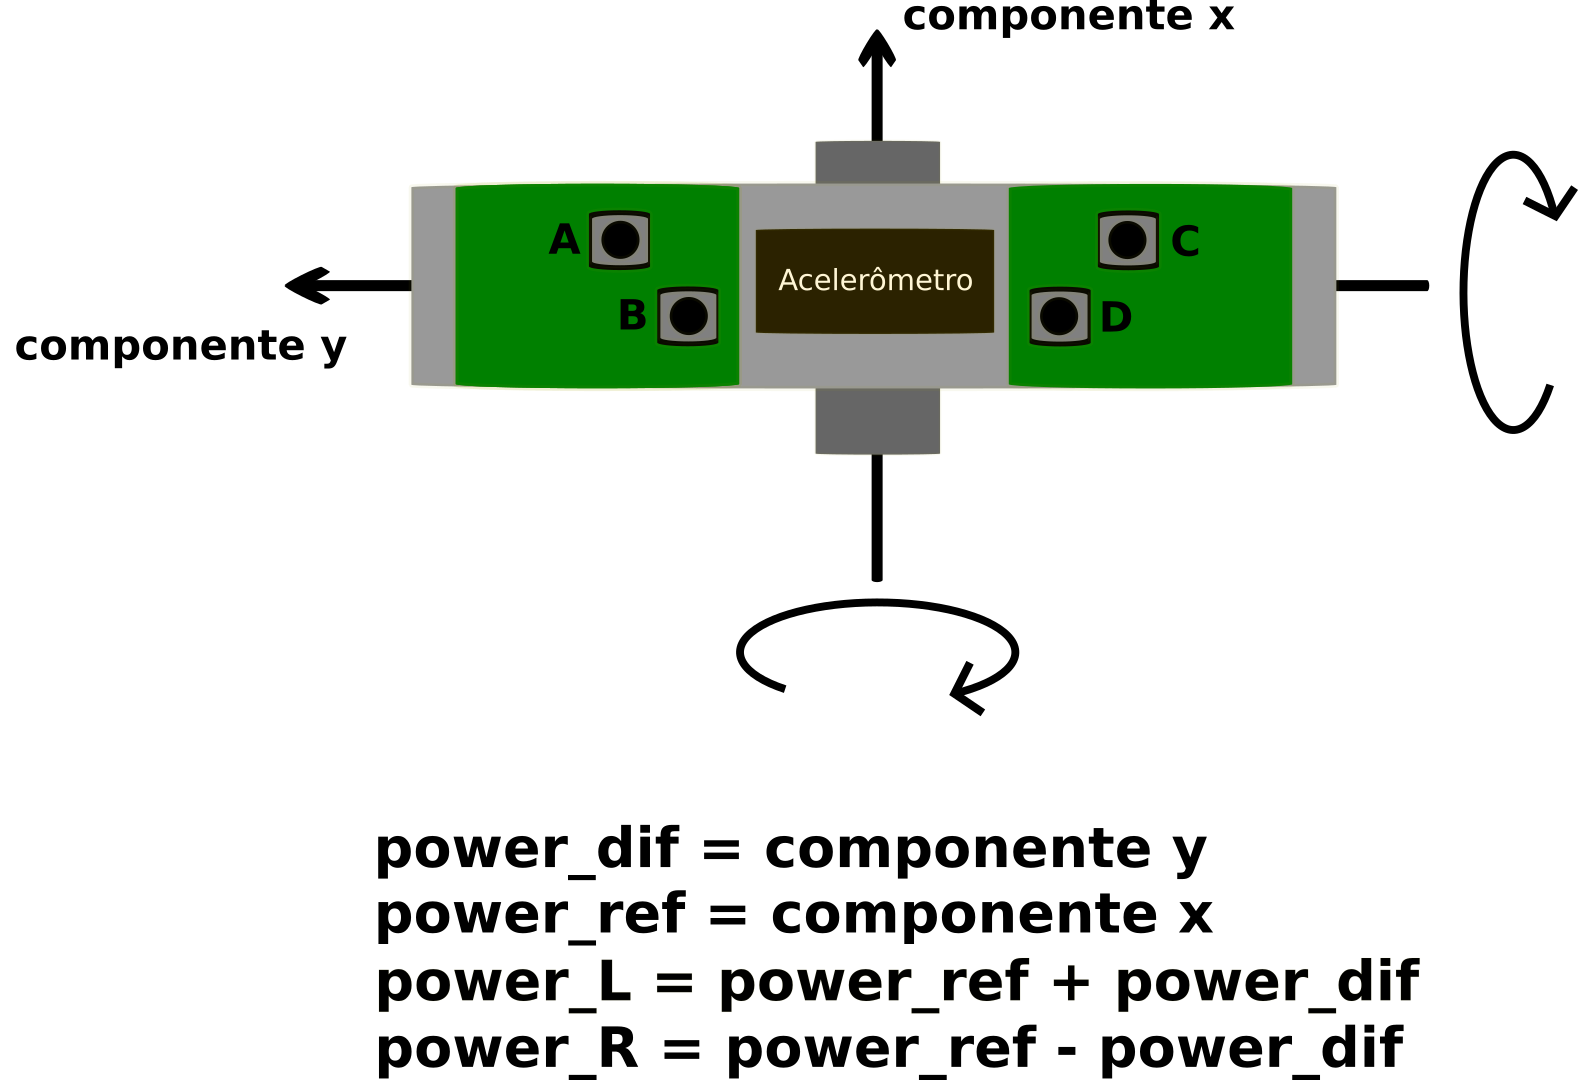
\includegraphics[width=1\textwidth]{./img/concepcao/controle_acelerometro.png}
\end{figure}
Fonte: \textit{Autor}

Botões na interface de controle, como os botões A, B, C e D na Figura \ref{fig:controle_acelerometro}, possibilitam mais funcionalidades.
Para que a interface de controle não fique acionando os motores enquanto não estiver sendo manuseada, os botões podem ser utilizados para isso. Dessa forma, se for programado que a interface de controle só irá enviar sinais se os botões estiverem sendo pressionados, não acontecerá acionamentos em quanto a interface de controle não estiver sendo manuseada.

\pagebreak

A energia da plataforma provem de um barramento 12 V. Um conversor \textit{buck} pode ser usador para criar um barramento de 5 V. Dessa forma é possível fornecer energia a sistemas que trabalham com alimentação de 5 V, como as placas \textit{Raspberry Pi}. 
Uma ponte H controlada pelo processador de tempo real pode regular a potência fornecida aos motores pelo barramento de 12 V. O arranjo descrito é ilustrado na Figura \ref{fig:mapa_pot}.  

\begin{figure}[!htb]
  \centering
  \caption{Mapa de potência.}
  \label{fig:mapa_pot}
  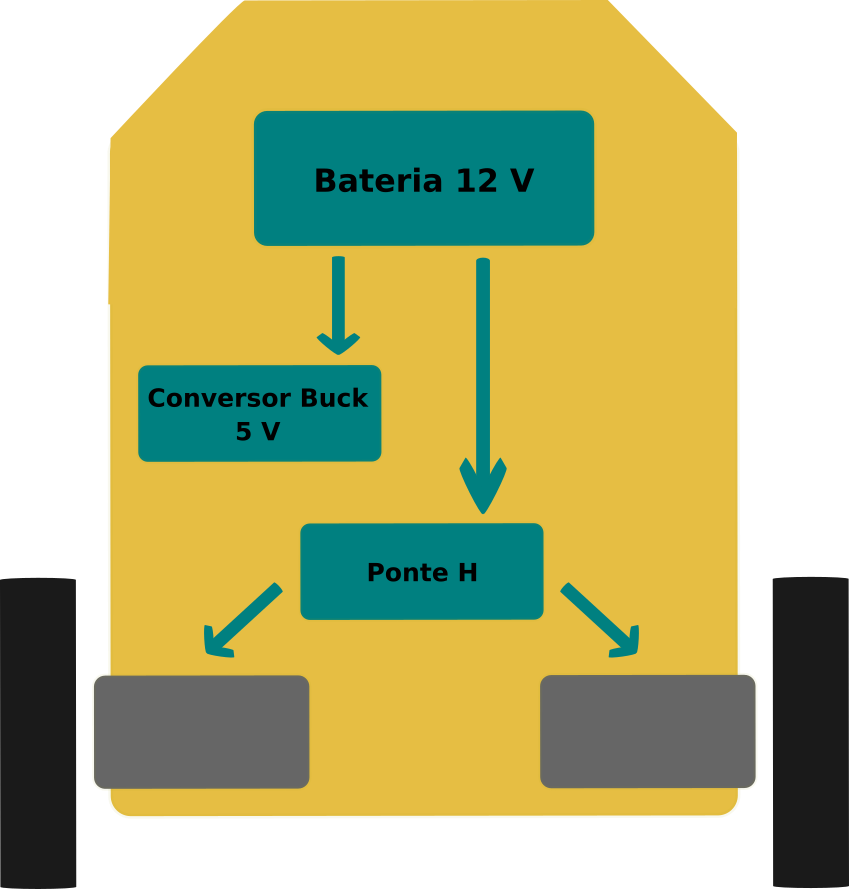
\includegraphics[width=0.7\textwidth]{./img/concepcao/mapa_pot.png}
\end{figure}
Fonte: \textit{Autor}

\pagebreak

\section{Concepção do sensor de distância baseado em visão estereoscópico}

O acoplamento de um par de câmeras permite, além dos algorítimos de visão monocular, o teste de algorítimos de visão estereoscópica.
Nesse trabalho serão testados um sistema de visão estéreo montado com duas \textit{webcams} e o sistema Microsoft Kinect. 
Ambos os sistemas, por meio do mapa de profundidade composto pelas imagens do par de câmeras, terão função de medir a distância frontal como apresentado na Figura \ref{fig:visao_estereo}.

\begin{figure}[!htb]
  \centering
  \caption{Sensor de Distância.}
  \label{fig:visao_estereo}
  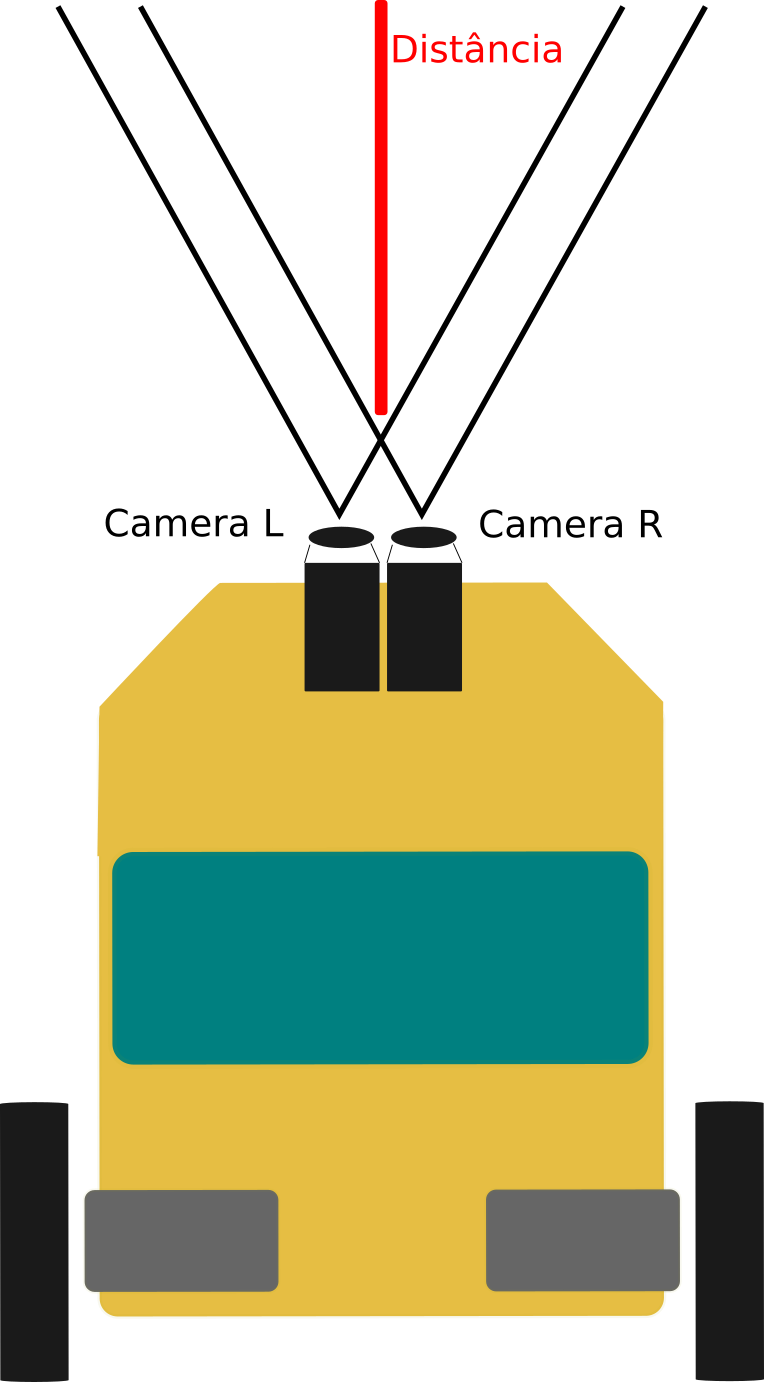
\includegraphics[width=0.5\textwidth]{./img/concepcao/visao_estereo.png}
\end{figure}
Fonte: \textit{Autor}

\pagebreak

\chapter{Projetos}

\section{Revisão da tecnologia disponível para o projeto}

Fundamentado no quesito disponibilidade do componente no DAELN (Departamento Acadêmico de Eletrônica), o \textit{hardware} escolhido tanto para o acionador dos motores quanto para o projeto da interface de controle foi o \textit{kit} de desenvolvimento \textit{Arduino Uno}. Esse carrega um microcontrolador \textit{AVR Atmega 328p} de \textit{8bits}.
Um \textit{Raspberry Pi 3 Model B+} havia disponível para ser usado como unidade principal de processamento, responsável por gerenciar os microcontroladores AVR e as câmeras. Esse também irá gerenciar a comunicação entre a rede \textit{wifi} e a plataforma além de fornecer a possibilidade de usar sua antena de comunicação \textit{Bluetooth}. Como fonte de energia foi utilizado um arranjo paralelo de bateria de chumbo-ácido de 12 V.
Um conversor estático do tipo \textit{buck} é responsável de gerar um barramento de tensão de 5 V a partir do barramento de 12 V onde as baterias estão conectadas. Haviam duas câmeras Logitec iguais que foram arranjadas em um sistema de visão estereoscópica e um sensor Microsoft Kinect. O Arranjo da plataforma é ilustrado na Figura \ref{fig:hardware_utilizado}. No caso da plataforma for esquipada com o sensor Kinect, esse deve ser alimentado com uma tensão de 12 V.

\begin{figure}[!htb]
  \centering
  \caption{\textit{Hardware} utilizado.}
  \label{fig:hardware_utilizado}
  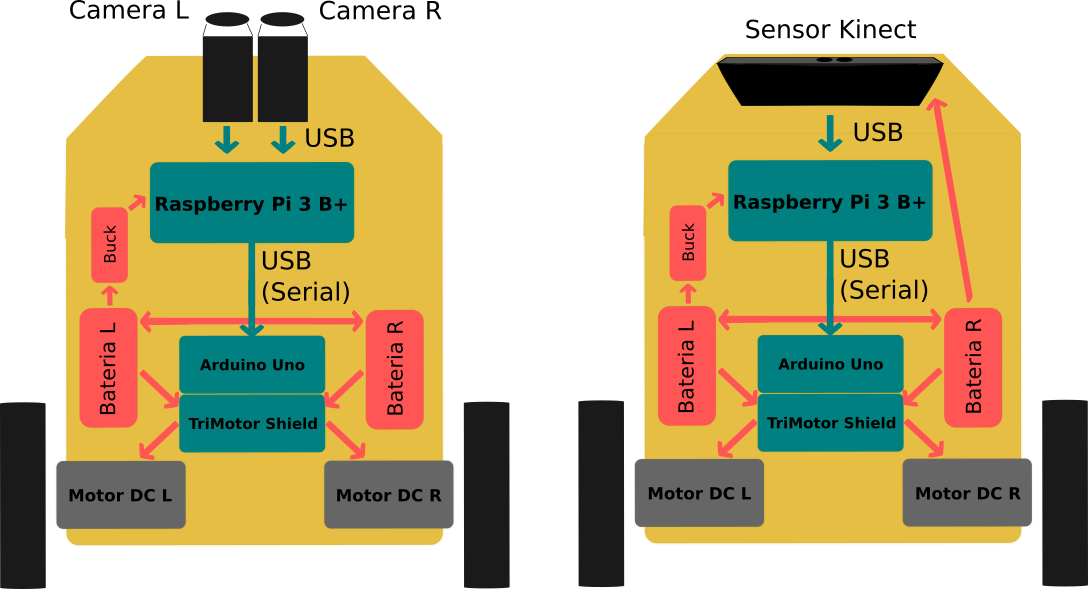
\includegraphics[width=1\textwidth]{./img/projeto/hardware_utilizado.png}
\end{figure}
Fonte: \textit{Autor}

\pagebreak

\begin{figure}[!htb]
  \centering
  \caption{\textit{Hardware} utilizado.}
  \label{fig:hardware_utilizado_controle}
  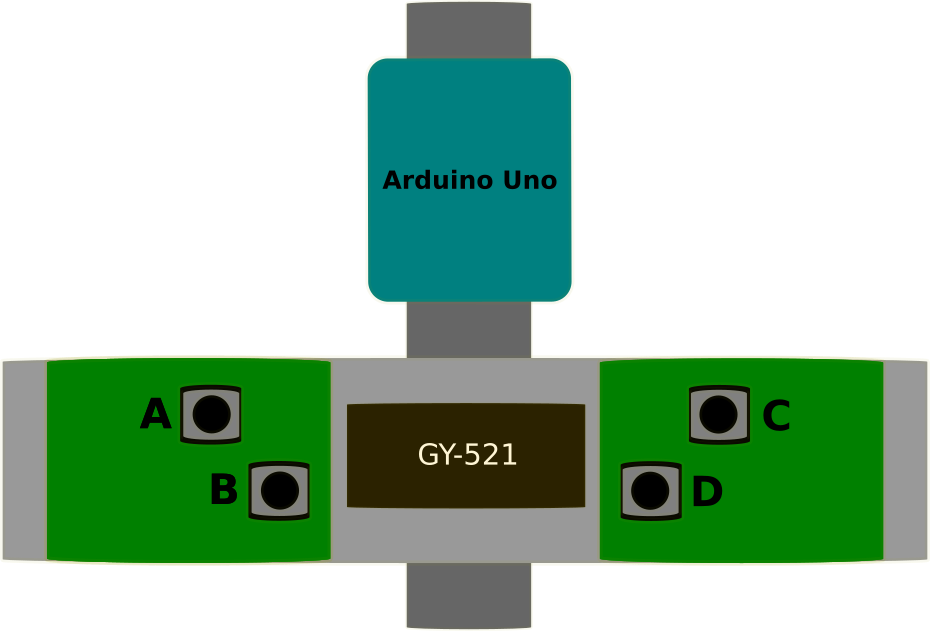
\includegraphics[width=1\textwidth]{./img/projeto/hardware_utilizado_controle.png}
\end{figure}
Fonte: \textit{Autor}

\pagebreak

Os componentes eletro-eletrônico necessários:
\begin{enumerate}[label=\alph*)]
    \item 1 placa \textit{Raspberry Pi 3 Model B+} 
    \item 2 placas \textit{Arduino Uno}
    \item 1 placas \textit{Tri Motor Shield}
    \item 2 Motores DC.
    \item 1 placas \textit{Conversor de Tensão Buck Boost Ajustável DC-DC}
    \item 2 Webcams Logitec
    \item 1 Sensor Kinect
    \item 1 Placa GY-521
    \item 1 Notebook
\end{enumerate}

\pagebreak

\begin{figure}[!htb]
  \centering
  \caption{Diagrama Elétrico.}
  \label{fig:diagrama_eletrico}
  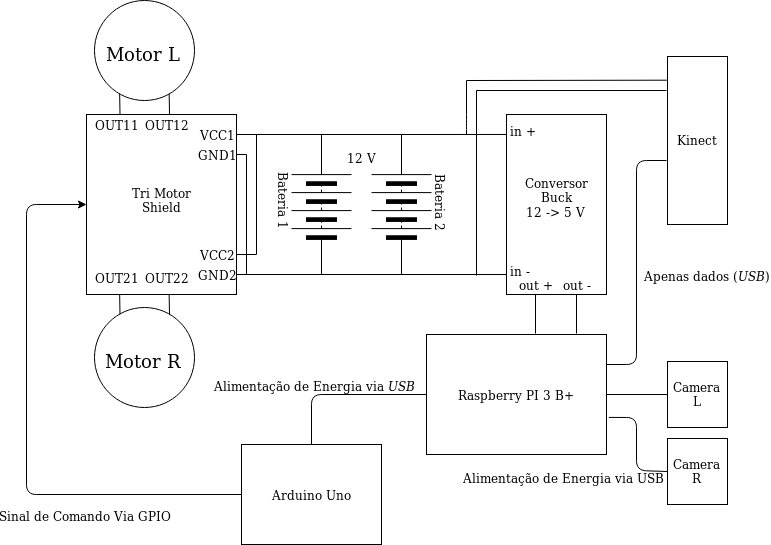
\includegraphics[width=1\textwidth]{./img/projeto/diagrama_eletrico.png}
\end{figure}
Fonte: \textit{Autor}
\pagebreak

\section{Projeto do controle}

\subsection{\textit{Hardware}}

Por meio da combinação de botões pressionados é possível acionar diferentes funcionalidades. 
A Figura \ref{fig:controle_acel} ilustra o acionamento da funcionalidade de controle do carro por meio do acelerômetro. O botão A pressionado faz com que o controle envie o sinal da componente y da gravidade medida pelo acelerômetro. 
O botão C pressionado faz com que a interface de controle envie o sinal da componente x. 
Logo um valor do tipo inteiro sem sinal de 8 bits é utilizado para representar a amplitude do sinal.
A polaridade do sinal de cada motor pode ser representada por um sinal booleano.
Como o valor máximo representado por uma variável de 8 bits é 255, a soma das amplitudes do sinal \textbf{power\_dif} e \textbf{power\_ref} não deve extrapolar esse valor. Logo quando ambos os botões A e C estiverem pressionados, o valor de amplitude do sinal das componentes da gravidade são divididos por dois. 

\begin{figure}[!htb]
  \centering
  \caption{Controle por meio do acelerômetro.}
  \label{fig:controle_acel}
  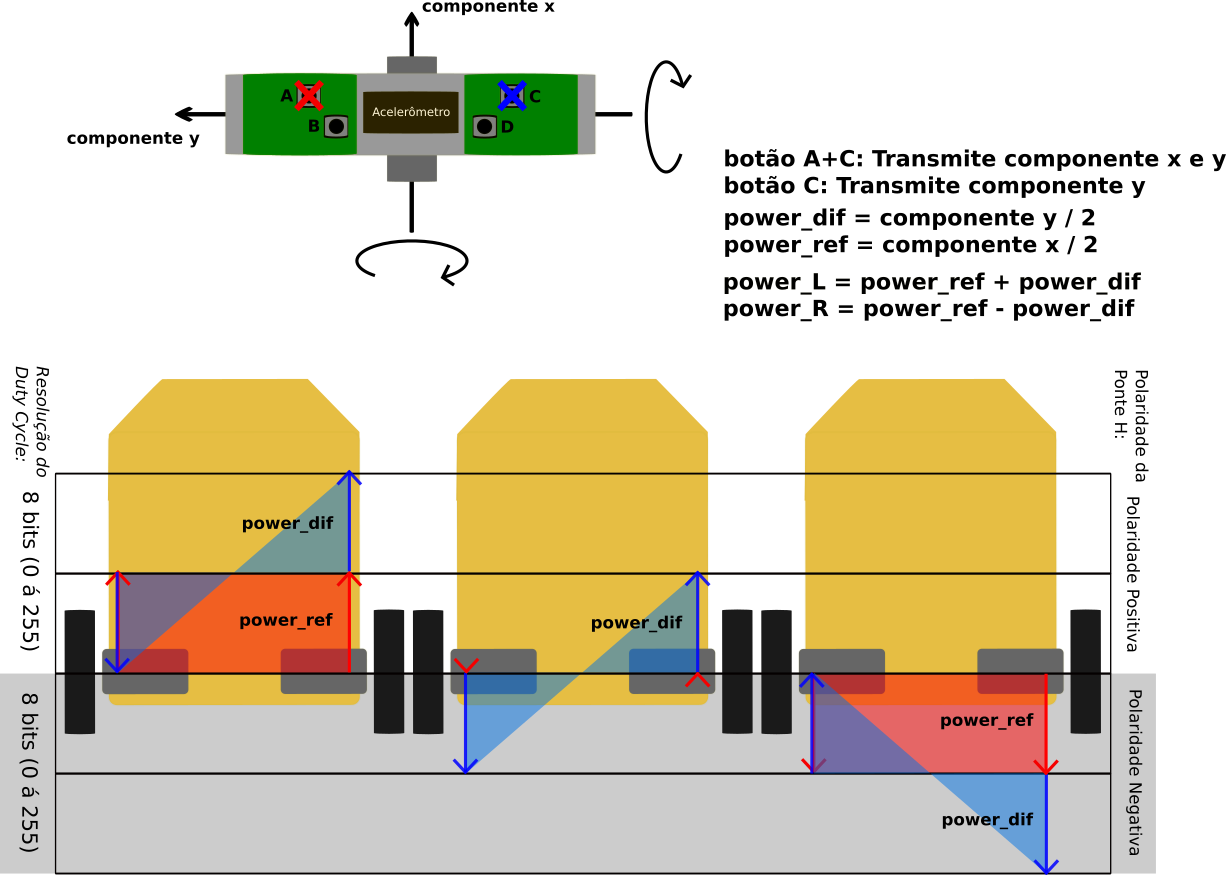
\includegraphics[width=1\textwidth]{./img/projeto/controle_acel.png}
\end{figure}
Fonte: \textit{Autor}

\pagebreak

Dessa forma , como indicado na Figura \ref{fig:controle_acel_individual}, é possível utilizar as componentes da aceleração da gravidade de forma independente. Como as componentes dessa vez não serão somadas, suas amplitude podem assumir valores maiores. No caso de utilizar apenas o botão A, o plataforma deve se mover em linha reta. 
Porém os motores não possuem mesmo rendimento.
Isso impossibilita um deslocamento em linha reta se for disponibilizada a mesma potência para ambos os motores. 
Uma margem de compensação \textbf{power\_comp}, no caso da Figura \ref{fig:controle_acel_individual}: $1/4$, da amplitude máxima do sinal pode ser deixada.
Dessa forma possibilitando implementado o sistema de controle afim de compensar a diferença de rendimento dos motores.

\begin{figure}[!htb]
  \centering
  \caption{controle acel individual.}
  \label{fig:controle_acel_individual}
  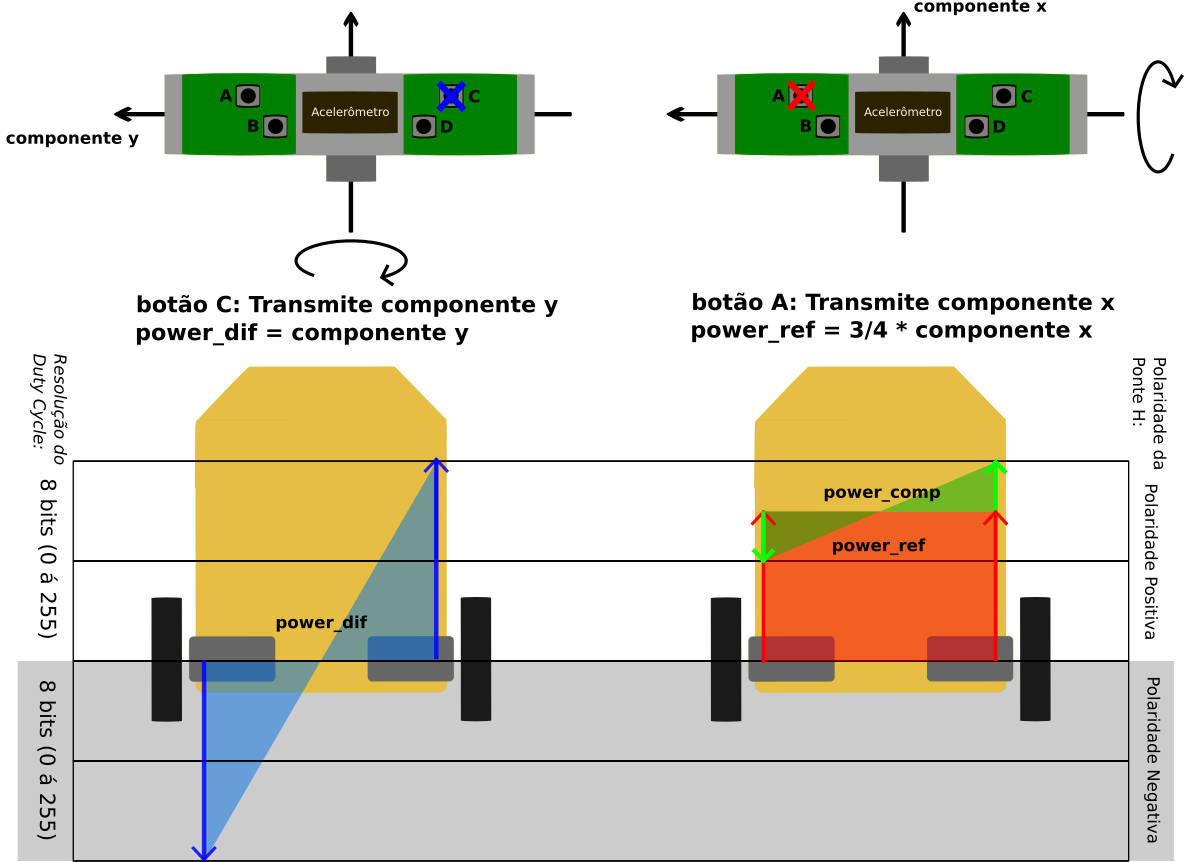
\includegraphics[width=1\textwidth]{./img/projeto/controle_acel_individual.png}
\end{figure}
Fonte: \textit{Autor}

\pagebreak

Como ilustrado na figura \ref{fig:controle_botao_up}.
Por meio dos botões B e D é possível acionar cada motor de forma independente afim de atribuir a máxima potência para cada motor. 
Dessa forma se torna possível controlar o carro apenas dosando a potência atribuída a cada motor ao pulsar os botões B e D.

\begin{figure}[!htb]
  \centering
  \caption{controle botao.}
  \label{fig:controle_botao_up}
  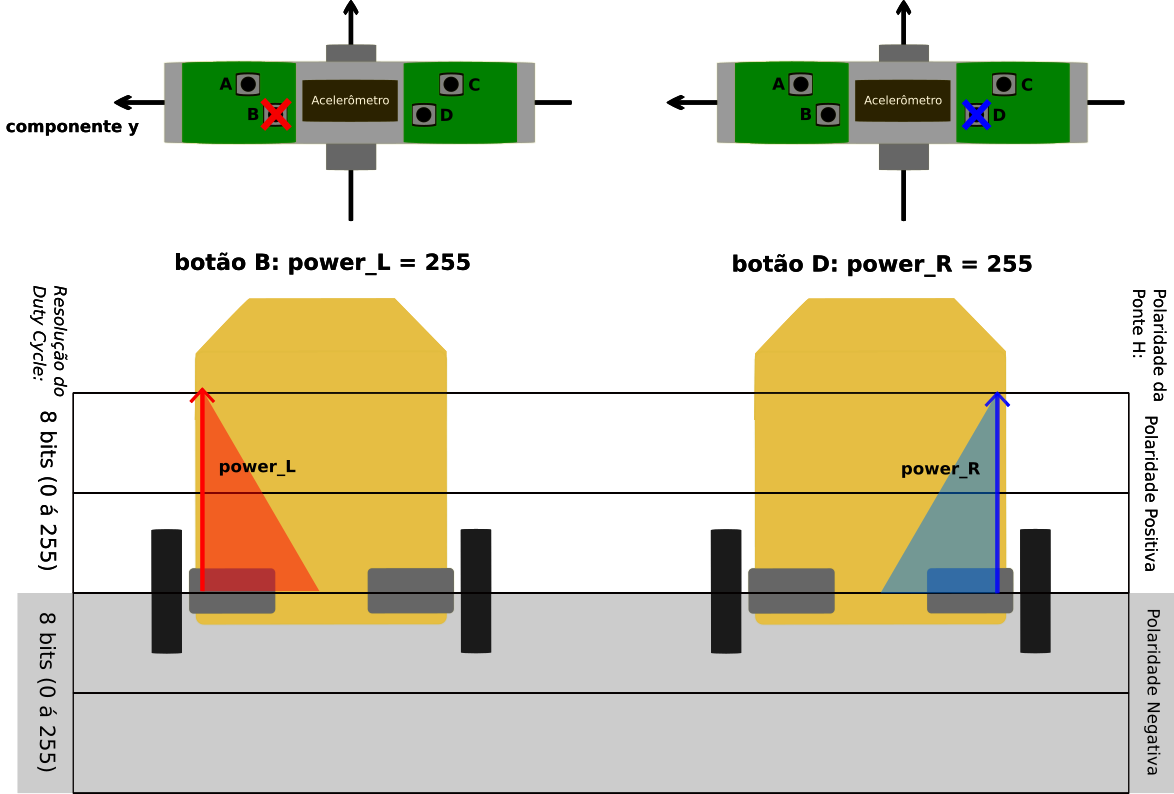
\includegraphics[width=0.75\textwidth]{./img/projeto/controle_botao_up.png}
\end{figure}
Fonte: \textit{Autor}

E a Figura \ref{fig:controle_botao_backward} ilustra que também á possibilidade de acionar os motores de forma inversa a Figura \ref{fig:controle_botao_up}.

\begin{figure}[!htb]
  \centering
  \caption{controle botao backward.}
  \label{fig:controle_botao_backward}
  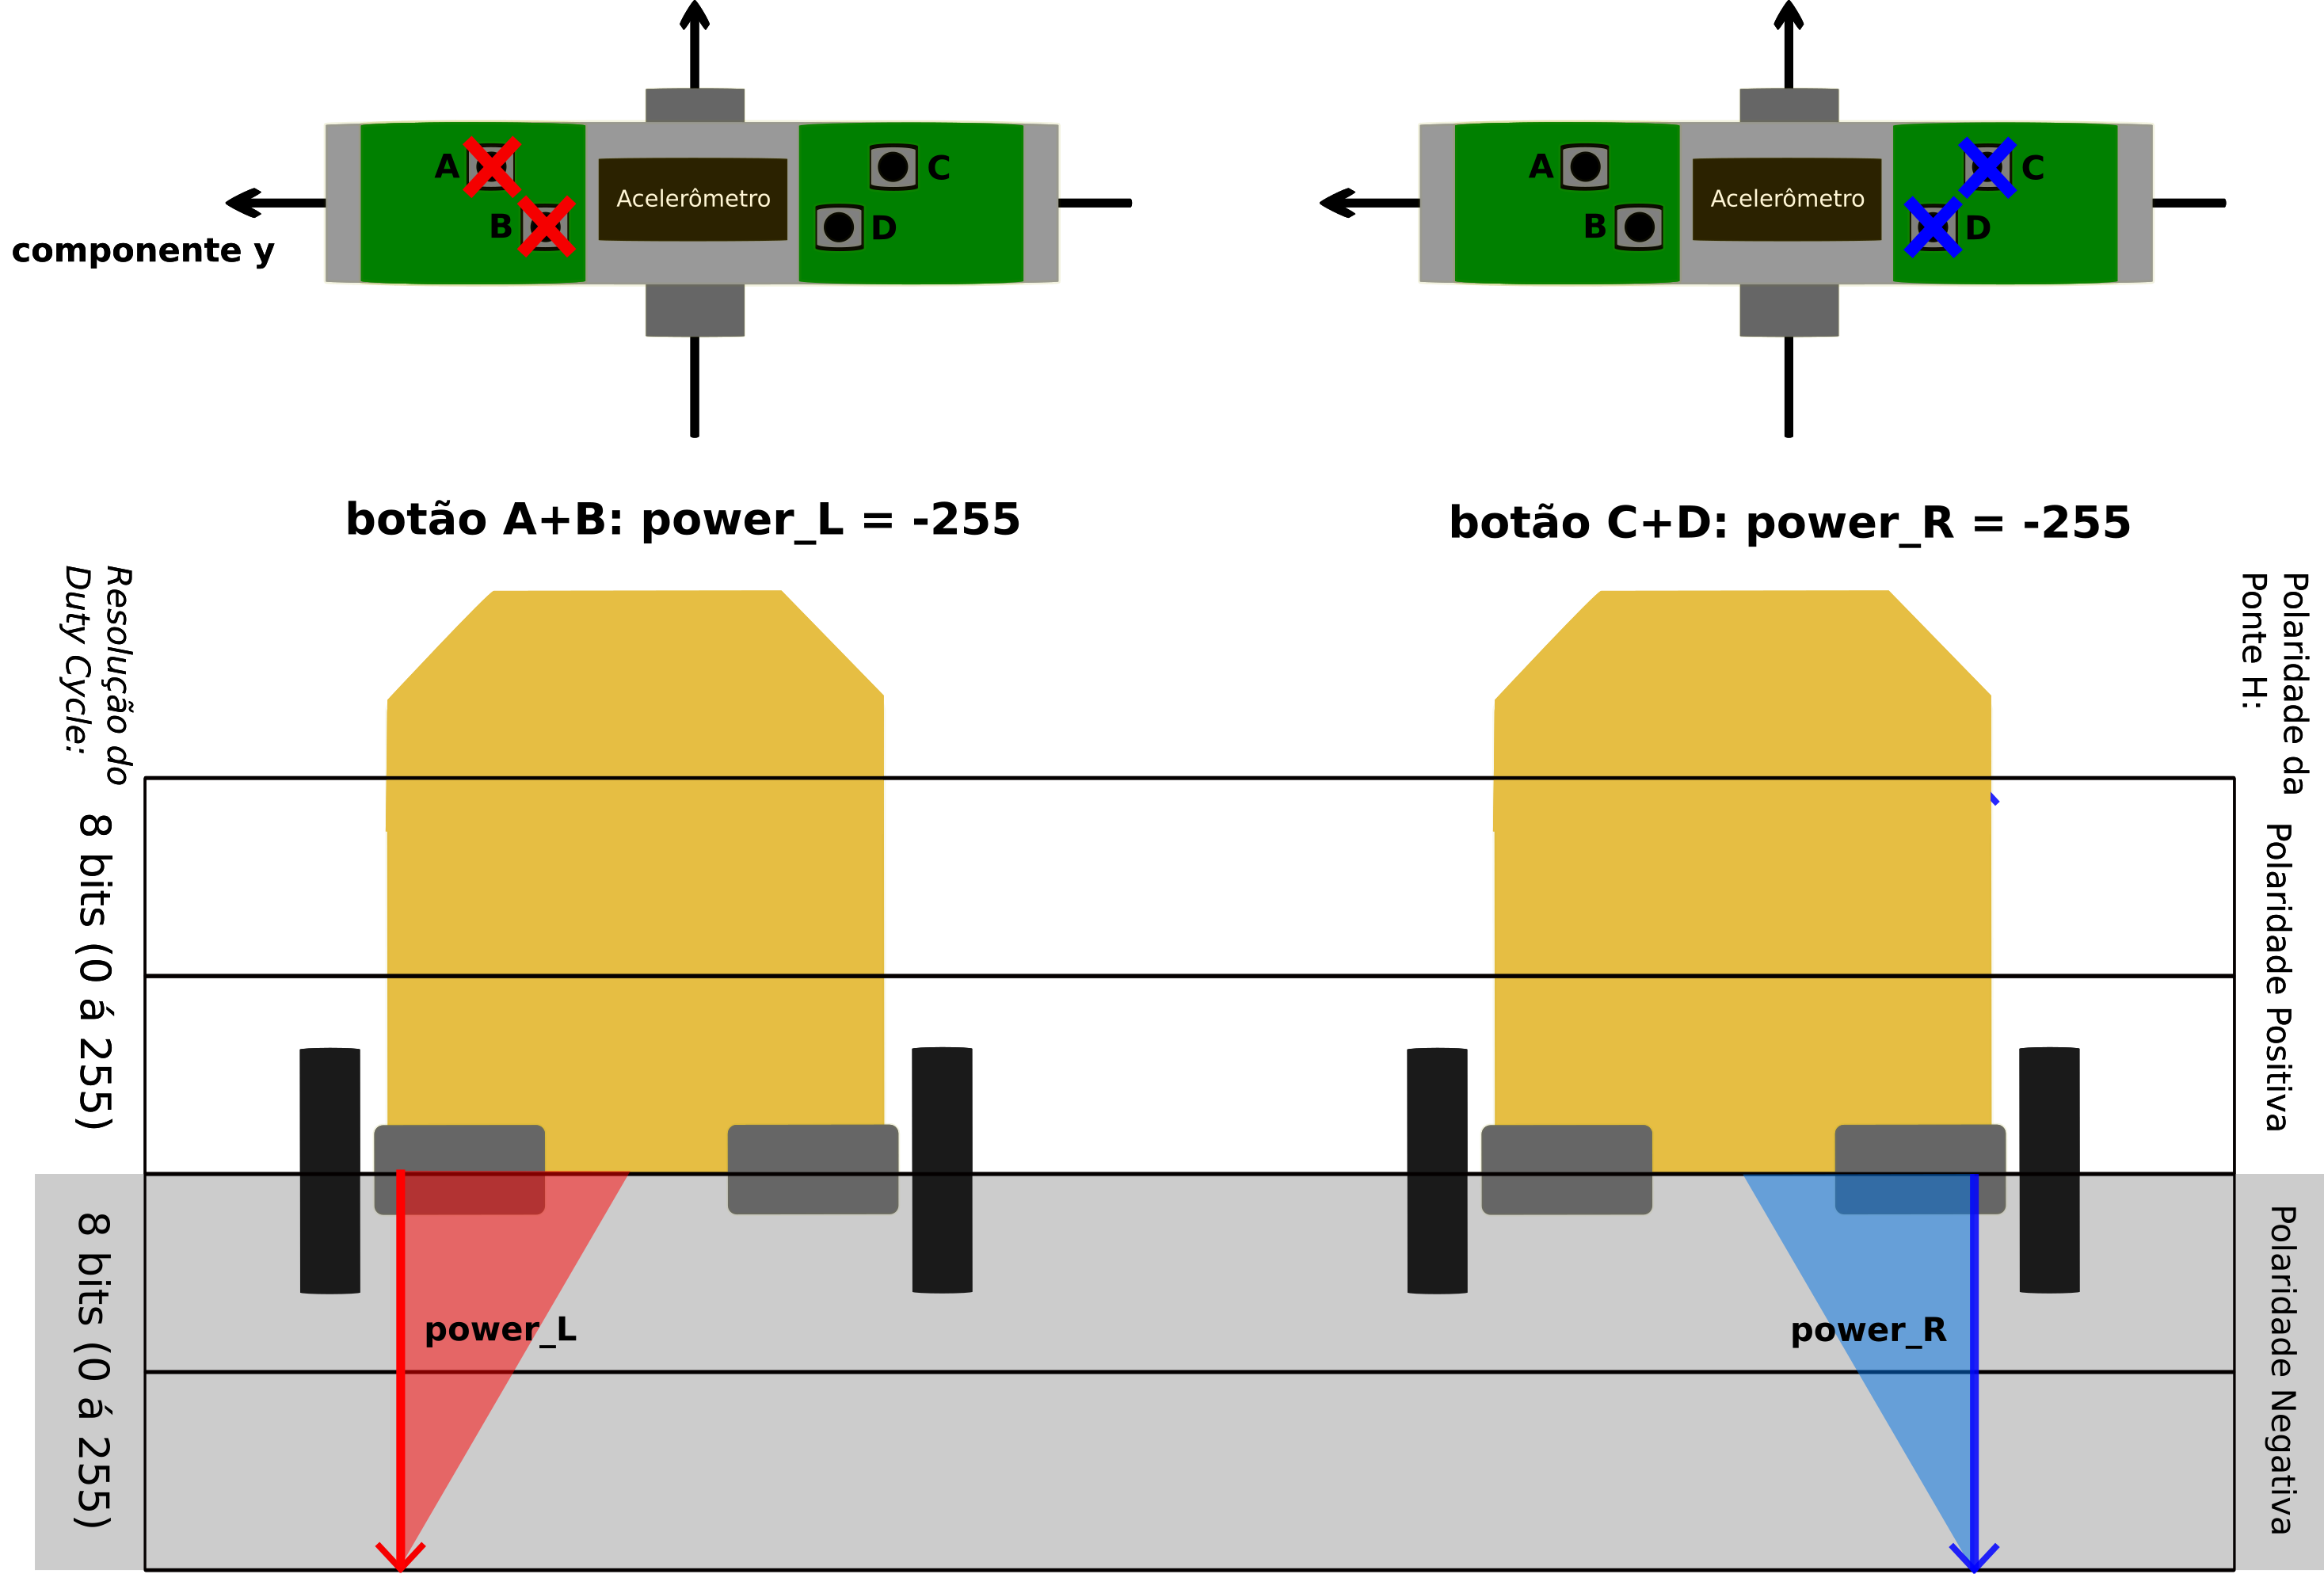
\includegraphics[width=0.75\textwidth]{./img/projeto/controle_botao_backward.png}
\end{figure}
Fonte: \textit{Autor}

\pagebreak

\subsection{\textit{Software}}

O sistema ROS permite a fácil comunicação entre nós de processamento via TCP/IP.
Logo, uma vez utilizando o sistema ROS, o sistema de controle pode ser divido como no grafo na Figura \ref{fig:rosnet_controle}. 
O nó \textit{/steering\underline{\hspace{.0625in}}wheel} e o \textit{/motor\underline{\hspace{.0625in}}driver} rodam cada um em uma placa Arduino Uno e o nó de controle roda Raspberry Pi. O pacote ROSSERIAL possibilita aos Arduinos Unos o acesso a camada de transporte por meio da porta serial. Dessa forma esses conseguem se comunicar via protocolo TCP/IP.

\begin{figure}[!htb]
  \centering
  \caption{Rede de Controle.}
  \label{fig:rosnet_controle}
  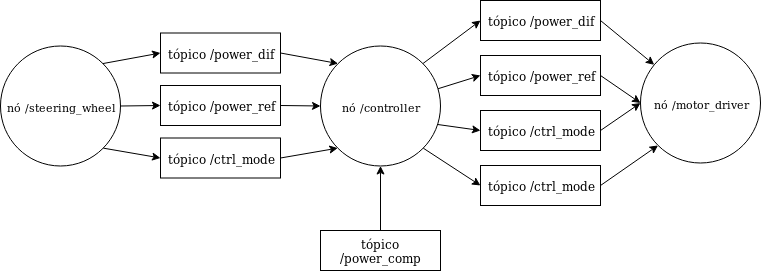
\includegraphics[width=1\textwidth]{./img/projeto/rosnet_controle.png}
\end{figure}
Fonte: \textit{Autor}

Apêndice \ref{app:steering_wheel}

\pagebreak

\section{Projeto do sensor de distância baseado em visão estereoscópico}
    \subsection{\textit{Hardware}}
    \pagebreak
    \subsection{\textit{Firmware}}    
    \pagebreak
    
\section{Projeto do procedimento de Teste}
    \subsection{Elaboração da tarefa teste}
    \pagebreak
    
\chapter{Implementações}

\section{Implementação da plataforma de prototipagem}
    \subsection{\textit{Hardware}}
    \pagebreak
    \subsection{\textit{Firmware}}
    \pagebreak
    
\section{Implementação do sensor de distância baseado em visão estereoscópico}
    \subsection{\textit{Hardware}}
    \pagebreak
    \subsection{\textit{Firmware}}
    \pagebreak
    
\section{Implementação do procedimento de teste}

\chapter{Operação}

\section{Teste da plataforma de prototipagem}
    \subsection{Análise do consumo de energia}
    \pagebreak
    
\section{Teste do sensor de distância baseado em visão estereoscópico}
    \subsection{Verificação dos valores de distância medidos}
    \pagebreak
    
    \subsection{Verificação dos tempos de processamento}
    \pagebreak
    
\section{Execução do teste}
    \subsection{Verificação do desempenho mediante ao procedimento de teste}
    \pagebreak
    
\chapter{Conclusão}

\begin{figure}[!htb]
  \centering
  \caption{Composição do \textit{hardware} do sistema.}
  \label{fig:robotCar_hardware}
  \includegraphics[width=0.95\textwidth]{./img/robotCar_hardware.png}
\end{figure}
Fonte: Autor

\pagebreak

Na Figura \ref{fig:robotCar_software} é apresentado a composição de \textit{softwares} que compõem o sistema. O ROS possibilita que o processamento de imagem pode ser executado parcialmente ou completamento pelo \textit{hardware} de maior pode computacional (que no caso é o computador).

\begin{figure}[!htb]
  \centering
  \caption{Composição do \textit{software} do sistema.}
  \label{fig:robotCar_software}
  \includegraphics[width=0.95\textwidth]{./img/robotCar_software.png}
\end{figure}
Fonte: Autor

\pagebreak

\chapter{Implementação}

\chapter{Operação}
  \includegraphics[width=0.7\textwidth]{./img/angulo_dif_power.png}

